%==========================================================================
\chapter{Godunov's Method For Non-Linear Schemes}\label{chap:godunov}
%==========================================================================


%============================================
\section{Notation}
%============================================


In the following chapters, numerical methods which discretize both space and time are discussed.
Space will be discretized in cells of equal size (or more precisely, of equal length, as only one
dimensional cases will be discussed). Integer indices describe their position. The following
convention is used: The index $0$ also represents the leftmost cell. Spatial indices are denoted as
subscripts. The time variable will be discretized in integer-valued time steps. The time steps may
have variable lengths from one time step to the next, but the time nevertheless progresses step by
step, which is denoted by integer superscripts.

Explicitly, the following notation is used:

\begin{itemize}
\item integer subscript: Value of a quantity at the cell, i.e. the center of the cell. Example:
$\U_i$, $\U_{i-2}$
\item non-integer subscript: Value at the cell faces (or interfaces), e.g. $\F_{i-\half}$ is
the flux at the interface between cell $i$ and $i-1$, i.e. the left cell as seen from cell $i$.
\item integer superscript: Indication of the time step. E.g. $\U ^ n$: State at time step $n$
\item non-integer superscript: (Estimated) value of a quantity in between time steps. E.g.
$\F^{n + \half}$: The flux at the middle of the time between steps $n$ and $n + 1$.
\end{itemize}




%============================================
\section{The Method}
%============================================


Armed with Riemann solvers for the Euler equations, we can now turn to solving other initial
value problems besides Riemann problems. Godunov's method is an excellent starting point to look
into some essential underlying concepts of finite volume methods. For simplicity, let's stick to
one dimensional problems to start with.


Let $\tilde{\U}(x, t^n)$ be some continuous state with $0 \leq x \leq L$ which we'd
like to evolve over time. The spatial domain is discretized into $N$ computing cells of regular
size $\Delta x = \tfrac{L}{N}$. Cell $i$'s center is located at $x_i = (i + \tfrac{1}{2}) \Delta
x$, while the cells' left and right boundaries are located at $x_{i - \half} = (i - 1) \Delta x$
and $x_{i+\half} = i\Delta x$, respectively. The state inside each cell is assumed to be piece-wise
constant, i.e. constant within the cell boundaries, which can be realized by taking integral
averages of the continuous state:

\begin{align}
    \U_i^n = \frac{1}{\Delta x} \int\limits_{x_{i-\half}}^{x_{i+\half}} \tilde{\U}(x, t^n) \de x \ .
\label{eq:godunov-averaging-state}
\end{align}

Obviously the states are allowed to vary from cell to cell. The piece-wise constant representation of
continuous data through integral averages as prescribed by eq.~\ref{eq:godunov-averaging-state} is
shown in  Fig.~\ref{fig:piecewise-constant}.

Godunov's method is based on the integral form of conservation laws, i.e.

\begin{align}
 \int\limits_{x_1}^{x_2} \int\limits_{t_0}^{t_1} \de x \de t \left[ \deldt \tilde{\U} + \deldx \F
\right] = 0
\end{align}

and as such allows for discontinuous solutions. Applying this integral form to the volume of a
single cell, i.e. $x_1 = x_{i-\half}$ and $x_2 = x_{i+\half}$ and between two times $t_0 = t^n$ and
$t_1 = t^{n+1}$ gives


\begin{figure}
    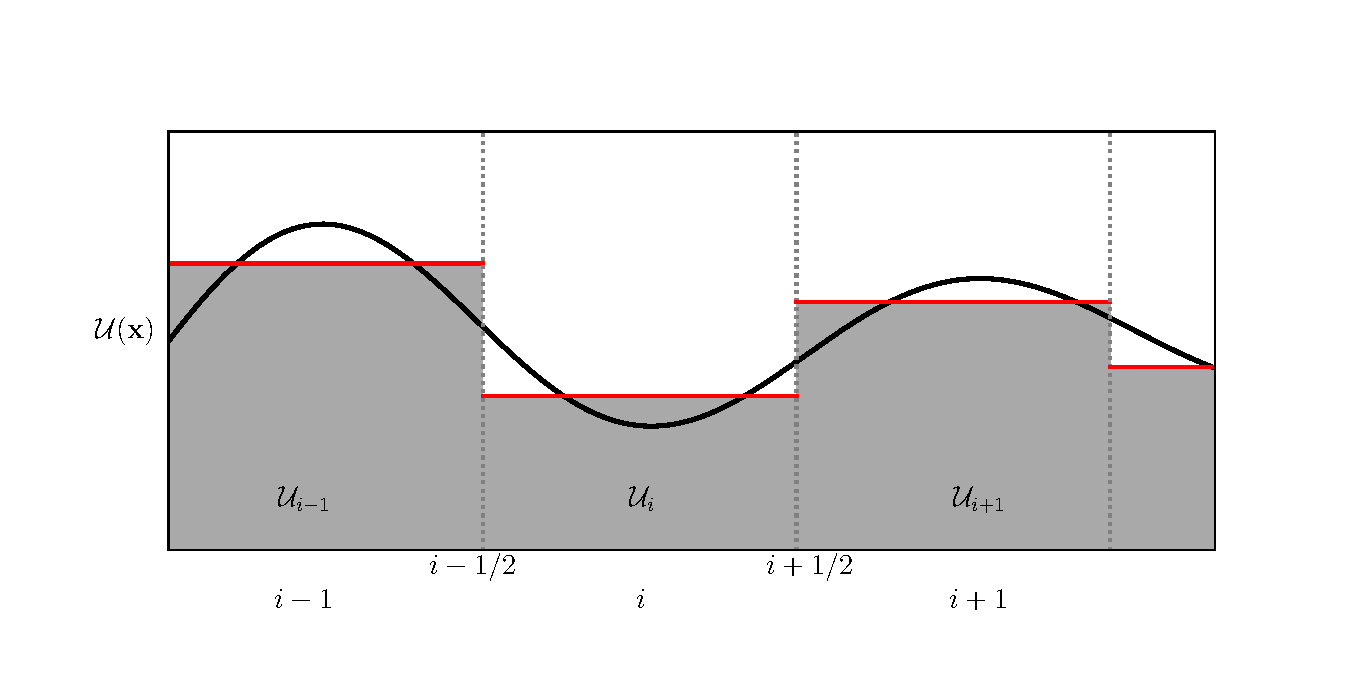
\includegraphics[width=\textwidth]{./figures/FV/piecewise_const.pdf}%
    \caption[A piece-wise constant representation of continuous data among cells.]
    {
A piece-wise constant representation (in red) of initially continuous data (black line)
among cells.
    }
\label{fig:piecewise-constant}
\end{figure}


\begin{align}
 \int\limits_{x_1}^{x_2} \tilde{\U}(x, t^{n+1}) \de x  =
 \int\limits_{x_1}^{x_2} \tilde{\U}(x, t^{n}) \de x  +
 \int\limits_{t^n}^{t^{n+1}} \F(\tilde{\U}(x_{i-\half}, t)) \de t -
 \int\limits_{t^n}^{t^{n+1}} \F(\tilde{\U}(x_{i+\half}, t)) \de t
\label{eq:conservation-law-integral-form}
\end{align}

At this point, we use our knowledge of the general structure of the solution of the Riemann problem
at the cell boundaries $x_{i \pm \half}$. At the left boundary, $x = x_{i-\half}$, the state
$\U(x_{i-\half}, t)$ for $t > 0$ is given by the solution of the Riemann problem with the left
state $\U_L = \U_{i-1}$ and the right state $\U_R = \U_{i}$ centered at the boundary $x =
x_{i-\half}$. The elementary wave solution of the Riemann problem tells us that as time evolves,
there will be three waves emanating from that point, separating the two initial states into four
constant states. The structure of the solution is shown in Figure~\ref{fig:riemann-solution}. What
Figure~\ref{fig:riemann-solution} also shows very well is that for all $t > 0$, the state at $x' =
0$
($x'$ being the $x$ coordinate in the frame of reference in Figure~\ref{fig:riemann-solution}, i.e.
of the centered Riemann problem) will remain constant: The only thing that varies over time is
the position of the wave fronts, which travel at constant speeds and are therefore straight lines on
the $x'-t$ plane. So once the state for $x' = 0$ is determined for $t > 0$, it will remain
constant. This is also true when $x' = 0$ is inside a rarefaction fan, as the state is determined
by the characteristics that satisfy $x'/t = 0$ (compare also the explicit solutions given in
eqns.~\ref{eq:rho-rarefaction-fan-left} ~-~\ref{eq:pressure-rarefaction-fan-right}). Therefore the
state $\U(x_{i-\half}, t^n)$ at the left cell boundary $x = x_{i-\half}$, which corresponds to the
center $x' = 0$ of the centered Riemann problem, will also be constant for all $t > 0$. The same
holds true for the right boundary $x = x_{i+\half}$ for the Riemann problem with left state $\U_L =
\U_i$ and the right state $\U_R = \U_{i+1}$.

Making use of the fact that the states at the cell boundaries $\U(x_{i \pm \half})$ are constant,
the corresponding fluxes $\F(\U(x_{i \pm \half}))$ are constant as well, and the integrals over
time in eq.~\ref{eq:conservation-law-integral-form} are trivially solved:


\begin{align}
 \int\limits_{t^n}^{t^{n+1}} \underbrace{\F(\tilde{\U}(x_{i-\half}, t))}_{\equiv \F_{i-\half}
= \CONST} \de t-
 \int\limits_{t^n}^{t^{n+1}} \underbrace{\F(\tilde{\U}(x_{i+\half}, t))}_{\equiv \F_{i+\half}
= \CONST} \de t &=
 \underbrace{(t^{n+1} - t^n)}_{\equiv \Delta t} \left[ \F_{i-\half} - \F_{i+\half}  \right] \\
 &= \Delta t  \left[ \F_{i-\half} - \F_{i+\half}  \right]
\end{align}

leaving us with

\begin{align}
 \int\limits_{x_1}^{x_2} \tilde{\U}(x, t^{n+1}) \de x  =
 \int\limits_{x_1}^{x_2} \tilde{\U}(x, t^{n}) \de x  +
 \Delta t  \left[ \F_{i-\half} - \F_{i+\half}  \right] \label{eq:godunov-intermediate-step}
\end{align}

Dividing eq.~\ref{eq:godunov-intermediate-step} by $\Delta x$, we obtain


\begin{align}
 \frac{1}{\Delta x} \int\limits_{x_1}^{x_2} \tilde{\U}(x, t^{n+1}) \de x  =
 \frac{1}{\Delta x}  \int\limits_{x_1}^{x_2} \tilde{\U}(x, t^{n}) \de x  +
 \frac{\Delta t}{\Delta x}  \left[ \F_{i-\half} - \F_{i+\half}  \right]
\end{align}

and we recognize the integral averages (eq.~\ref{eq:godunov-averaging-state}), allowing us to write
the final form of Godunov's scheme:

\begin{align}
\boxed{
 \U^{n+1}_i = \U^{n}_i +
 \frac{\Delta t}{\Delta x}  \left[ \F_{i-\half} - \F_{i+\half}  \right]  \label{eq:godunov-scheme}
}
\end{align}




It is noteworthy that this is an exact solution to a piece-wise constant initial state. More
sophisticated cases, where assumptions of the states to be non-constant over the duration of
a time step, or for the states to be non-constant over the volume of a cell (e.g. a piece-wise
linear reconstruction instead of a piece-wise constant one) are relaxed, will be the topic of
Chapter~\ref{chap:higher-order-schemes}.

Something that was glanced over so far is that we assumed that the states and therefore the fluxes
at the cell boundaries remain constant indefinitely. While in theory that is true for isolated
Riemann problems that don't experience any outside perturbations nor influences, in this scenario
we have a collection of Riemann problems that are all a cell width $\Delta x$ apart from each
other. While the states at the boundaries, which represent the center of the Riemann problem,
remain constant in an isolated case, the waves emanating from that origin propagate over time, and
eventually cross the distance $\Delta x$ both towards the left and the right. Once they do, the
states at the distance $\Delta x$ from the origin will change. However, those are also the
positions of other cell boundaries, which we used as the origins for other Riemann problems and
assumed to remain constant. Clearly in this case the assumption of constancy of the states at cell
boundaries is violated. In order to prevent this violation from occurring, we must impose a
condition: The time step size $\Delta t$ must not be large enough for a wave to travel the distance
$\Delta x$, i.e.

\begin{align}
 \Delta t \leq \frac{\Delta x}{S_{max}^n}
\end{align}

where $S_{max}^n$ is the maximal wave speed among all waves emanating from the solutions of the
Riemann problems at each cell boundary. This condition is called the Courant-Friedrichs-Levy (CFL)
condition, and is usually expressed as

\begin{align}
 \Delta t = C_{CFL} \frac{\Delta x}{S_{max}^n}, \quad\quad C_{CFL} \in [0, 1) \label{eq:godunov-cfl}
\end{align}

$C_{CFL}$ is often referred to as the ``Courant number''.

Some more points need to be raised regarding the limitation of the time step size $\Delta t$.
Firstly, while the straightforward argumentation to prohibit waves from reaching adjacent cell
boundaries works for the comparatively simple Godunov scheme, matters can get more complicated for
higher order schemes and when more than one dimension is treated. In addition to physical
arguments, further restrictions must be included in order to ensure the stability of the scheme.
``Stability'' in this context refers to ensuring that spurious oscillations around discontinuities
such as shocks don't develop, as these oscillations can grow exponentially and quickly lead to
positive and negative infinite values in the solution. The development of oscillations around
discontinuities is a consequence of extending the method to higher orders of accuracy, and will be
discussed in Chapter~\ref{chap:higher-order-schemes}.

Doing proper stability analyses of the methods presented in this work would go way beyond the
scope of this thesis. To make matters worse, in more contrived cases like for higher order methods
and non-linear conservation laws, a rigorous proof of stability is not available to date. In
practice, the findings from simpler cases like linear conservation laws are applied to non-linear
ones as well, and are known to yield adequate results. Nevertheless, to provide an impression of how
stability analysis can be done, the outlines of two well-known methods of stability analyses are
given below:

\begin{itemize}
 \item The \emph{Von Neumann Stability Analysis} approach looks into the Fourier transform of the
underlying conservation law that is to be solved, and looks how the solution of the numerical method
evolves in Fourier space. Stability conditions are found by requiring that the solution in Fourier
space mustn't grow exponentially, but remain bounded for all times, and by ensuring that the phase
doesn't allow for too high propagation velocities.

\item The \emph{Lax-Richtmeyer Stability Analysis} relies on comparing the error resulting from the
numerical method being applied to a conservation law to the exact solution of the conservation law
at each time step. Since the method is applied repeatedly as the simulation progresses in order to
advance the initial state in time, the errors accumulate and propagate each time step. The stability
criteria arise from the requirement for the (cumulative) error to remain bounded.

\end{itemize}




Secondly, depending on the method, the exact wave speeds may not always be known. In Godunov's
method, where only a single Riemann problem is solved, the correct solution can be obtained, but
this is not always possible in higher order methods. Instead, an approximate estimate can be used. A
reliable choice is

\begin{align}
	S^n_{max} = \max_i\{ |v_i^n| + c_{s,i}^n \} \label{eq:wavespeed-estimate-godunov}
\end{align}

This estimate may underestimate the shock speeds (compare to eqns.~\ref{eq:shock-left-speed} and
\ref{eq:shock-right-speed}), but a reasonable choice of $C_{CFL}$ can ensure that no instabilities
occur. A value of $C_{CFL} \lesssim 0.8 - 0.9$ is recommended.


To conclude the chapter on Godunov's method, let's explicitly write down the algorithm to evolve a
system from some $t_{start}$ to some $t_{end}$:


\algo{Evolving A System From $t_{start}$ To $t_{end}$ Using Godunov's Method}
{
To start, set $t_{current} = t^0 = t_{start}$ and set up the initial states $\U_i^0$ for
each cell $i$.\\[.5em]
%
While $t_{current} < t_{end}$, solve the $n$-th time step:\\[.5em]
%
\indent~~~~Compute inter-cell fluxes: For every cell pair $(i, i+1)$, solve the Riemann \\
%
\indent~~~~~~~~problem to find the flux
$\F^n_{i+\half} = \F(\U_i^n, \U_{i+1}^n)$. \\[.5em]
%
\indent~~~~Find the maximal permissible time step $\Delta t$ using eq.~\ref{eq:godunov-cfl} \\[.5em]
%
\indent~~~~Find the updated states $\U_i^{n+1}$ using eq.~\ref{eq:godunov-scheme} \\[.5em]
%
\indent~~~~Update the current time: $t_{current} = t^{n+1} = t^n + \Delta t$
}













%==============================================================================
\section{Applications of Godunov's Method}\label{chap:godunov-application}
%==============================================================================

\begin{figure}
    \centering
    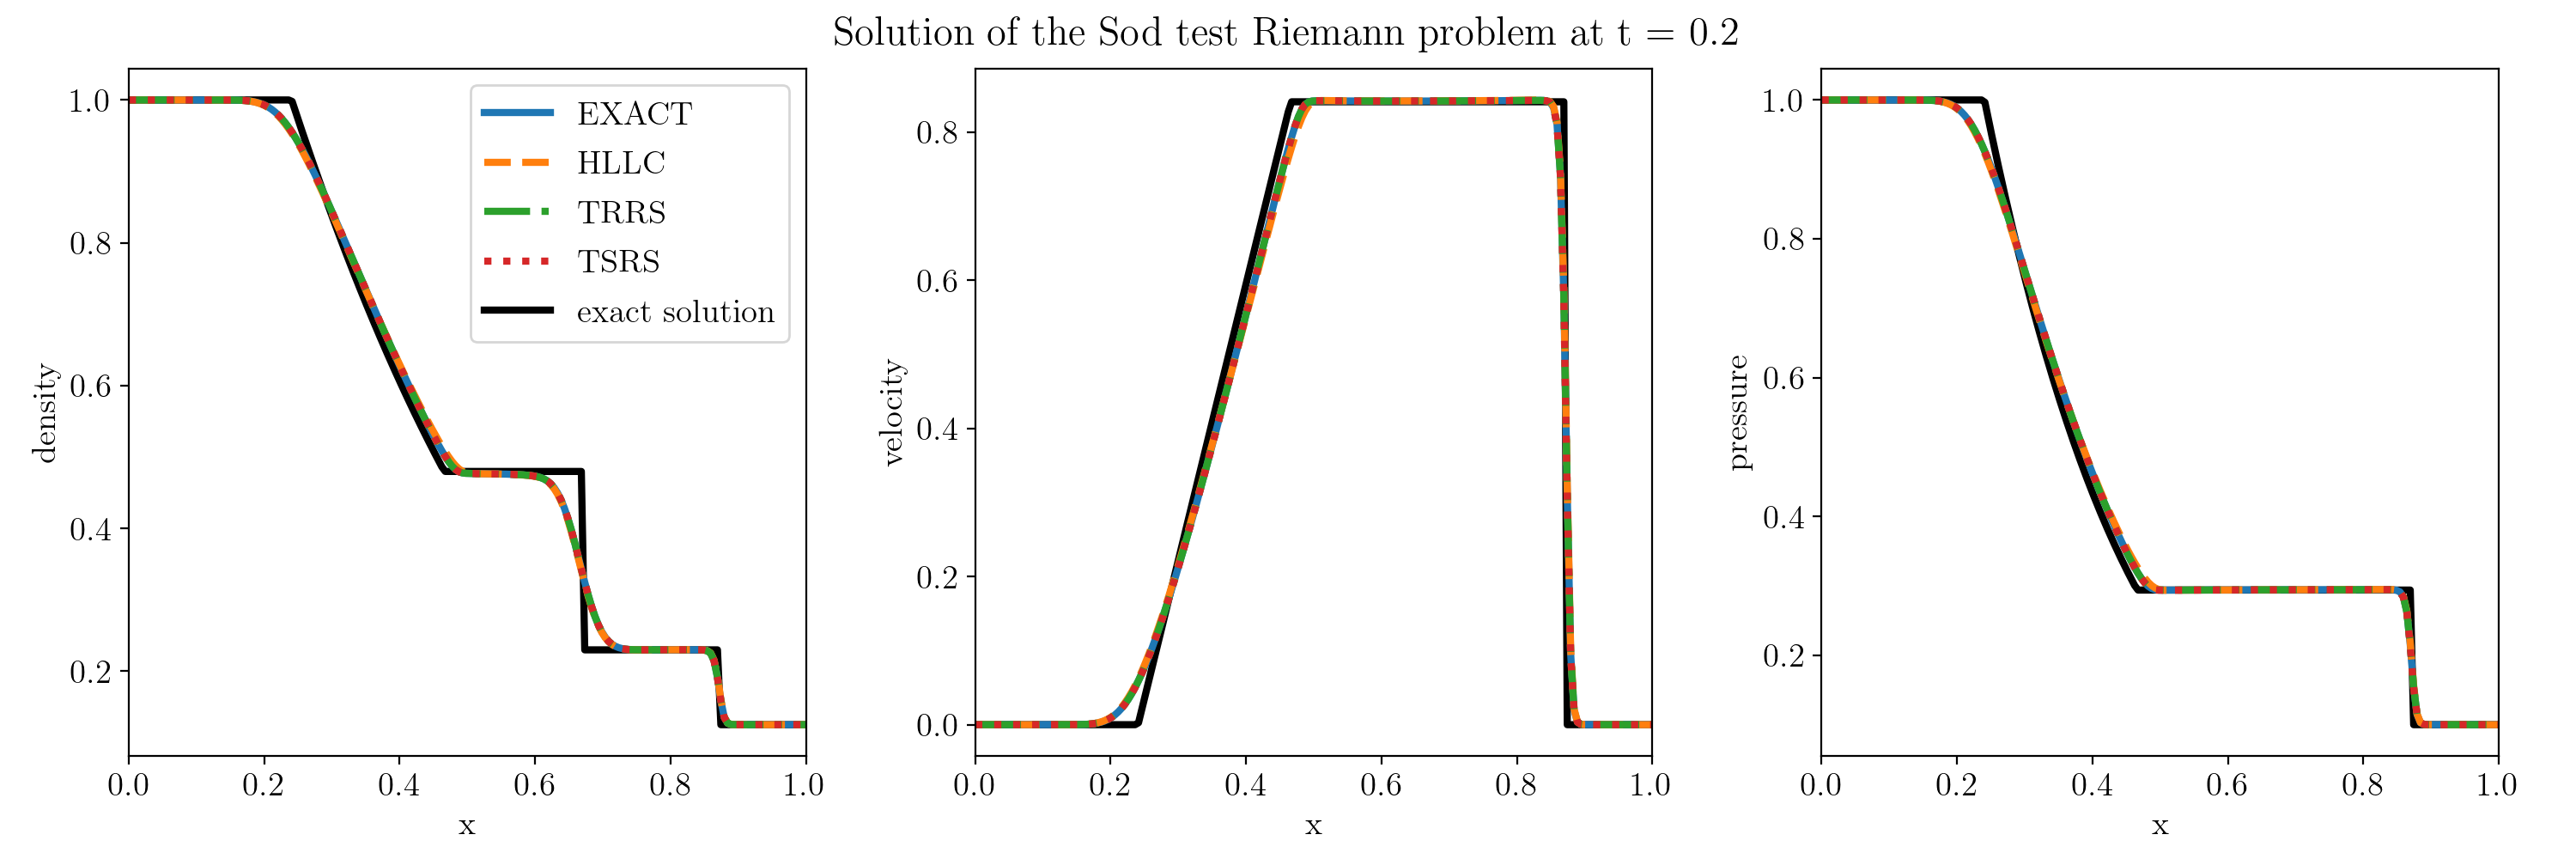
\includegraphics[width=\textwidth]{
    ./figures/FV/godunov_euler/GODUNOV-sod_test-1D.png} %
    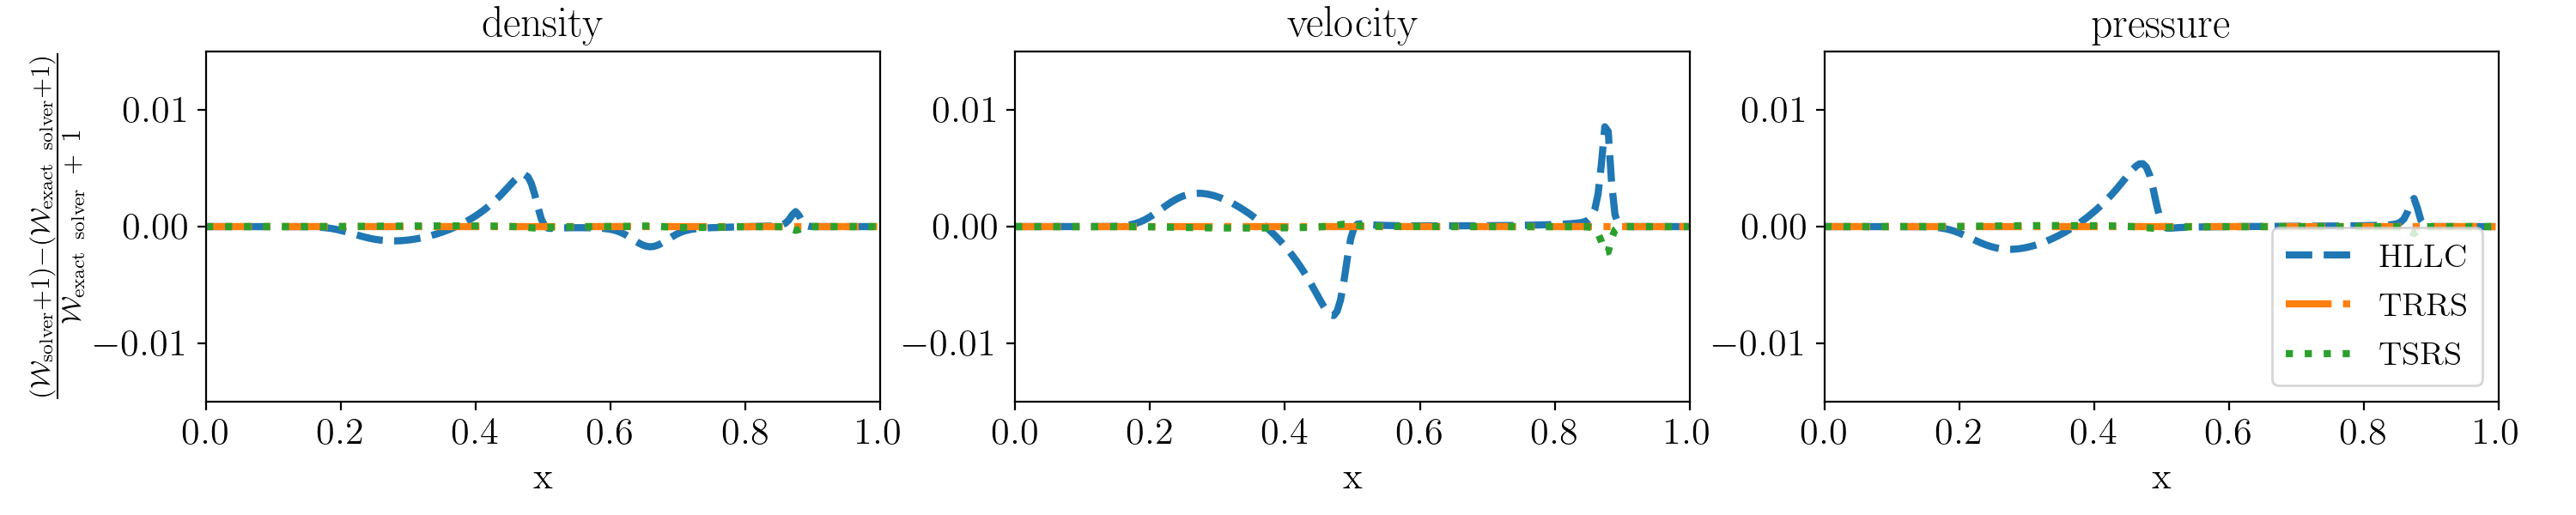
\includegraphics[width=\textwidth]{
    ./figures/FV/godunov_euler/GODUNOV-sod_test-differences-1D.png} %
    \caption[Sod test using Godunov's method]{
Top: The solution to the Sod test (eq. \ref{eq:sod-test-ICs}) using Godunov's method with the exact,
TRRS, TSRS, and HLLC Riemann solver, respectively, and the exact solution of the problem.
The solution consists of a left-facing rarefaction and a right facing shock. \\
Bottom: The relative differences of the solution of approximate Riemann solvers compared to the
solution using the exact Riemann solver with Godunov's method. The relative differences are
computed with all primitive quantities $\W = (\rho, v, p)$ being increased by 1 to avoid
divisions by zero.
    }%
    \label{fig:godunov-sod-test}
\end{figure}
%
\begin{figure}
    \centering
    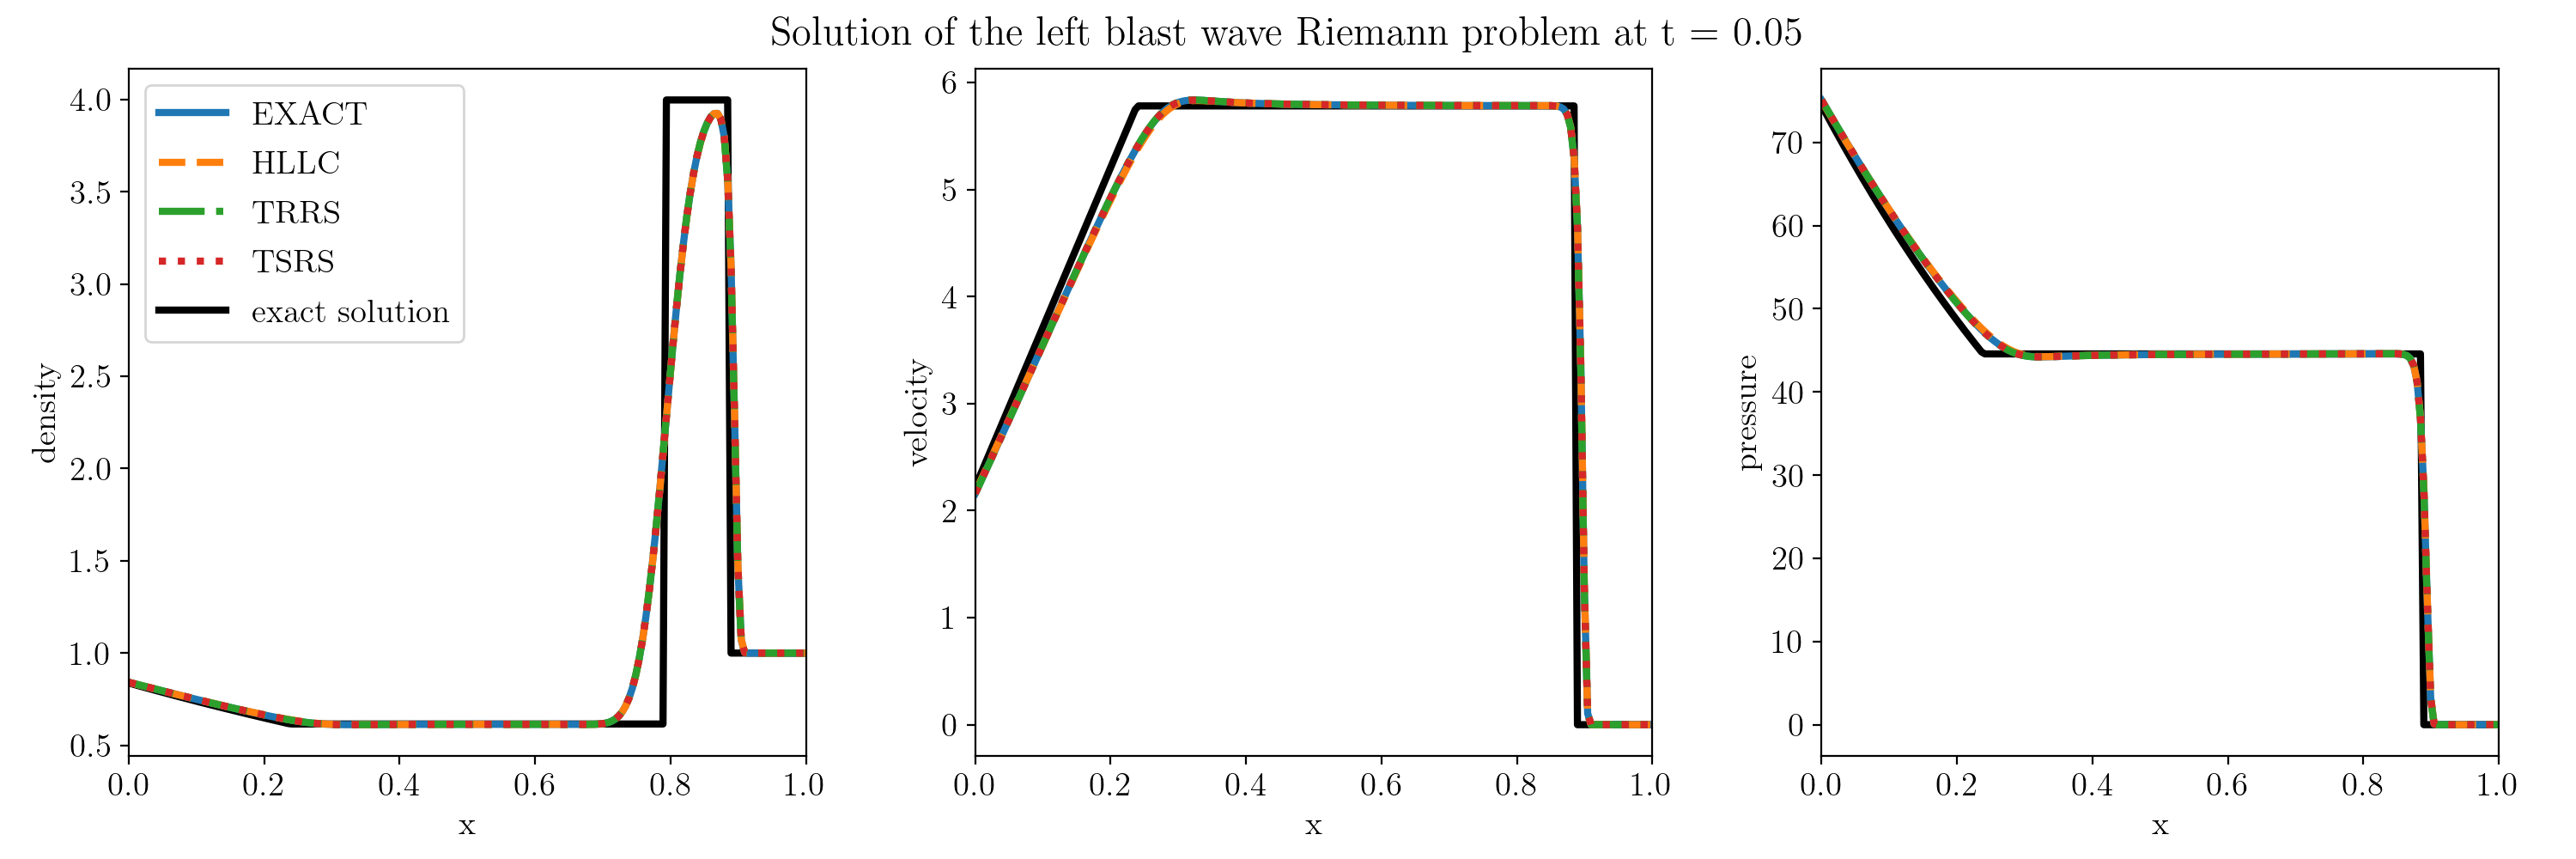
\includegraphics[width=\textwidth]{
    ./figures/FV/godunov_euler/GODUNOV-left_blast_wave-1D.png} %
    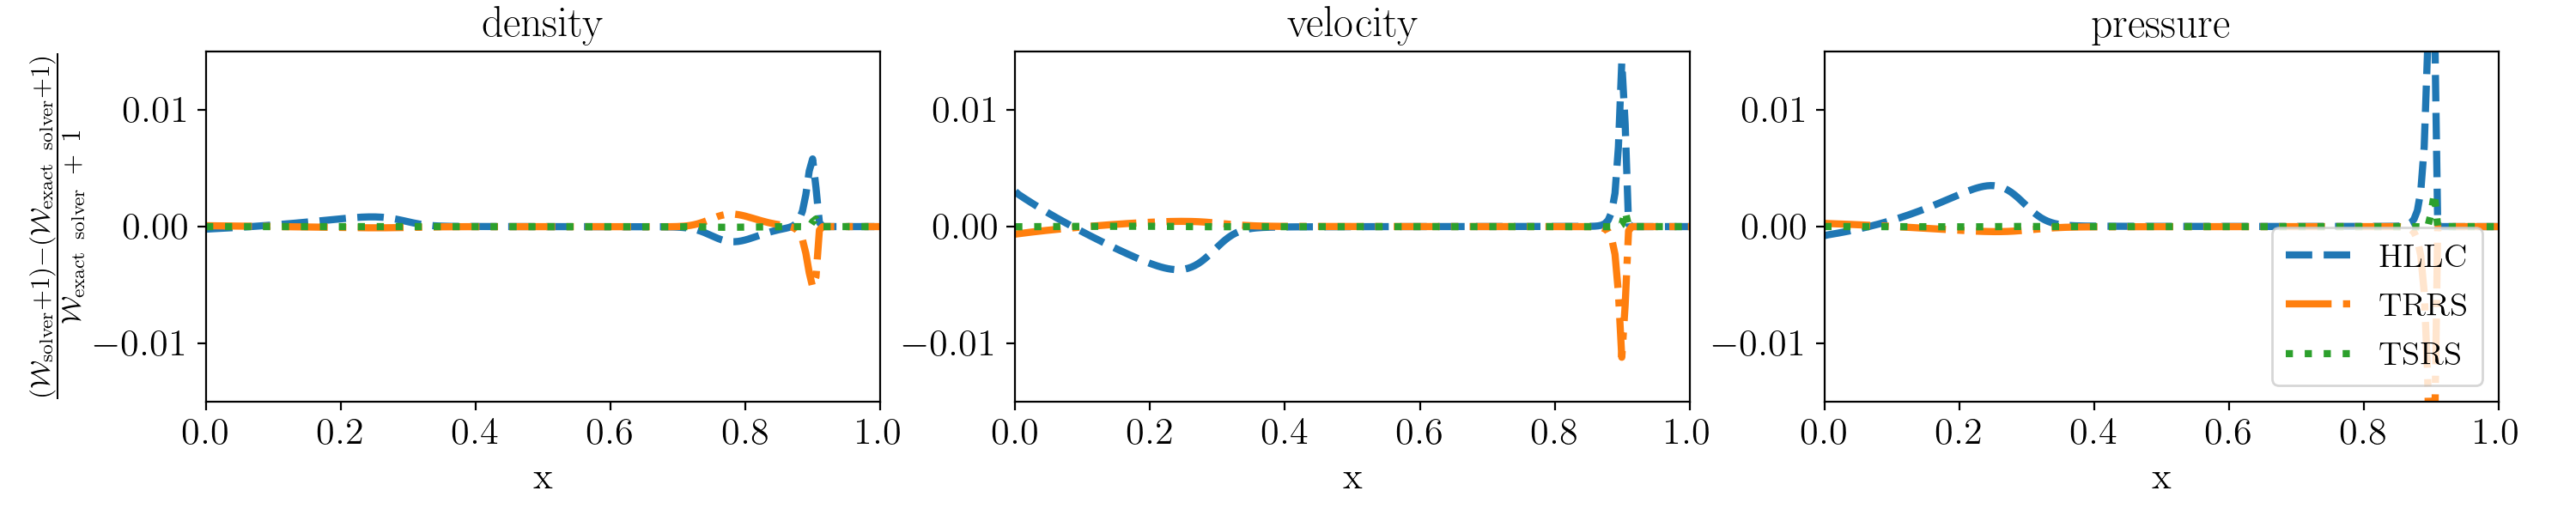
\includegraphics[width=\textwidth]{
    ./figures/FV/godunov_euler/GODUNOV-left_blast_wave-differences-1D.png} %
    \caption[Left blast wave solution using Godunov's method]{
Top: The solution to the left blast wave test (eq. \ref{eq:left-blast-wave-ICs}) using Godunov's
method with the exact, TRRS, TSRS, and HLLC Riemann solver, respectively, and the exact solution
of the problem.  The solution consists of a left-facing rarefaction and a right facing shock. \\
Bottom: The relative differences of the solution of approximate Riemann solvers compared to the
solution using the exact Riemann solver with Godunov's method. The relative differences are
computed with all primitive quantities $\W = (\rho, v, p)$ being increased by 1 to avoid
divisions by zero.
    }%
    \label{fig:godunov-left-blast-wave}
\end{figure}
%
\begin{figure}
    \centering
    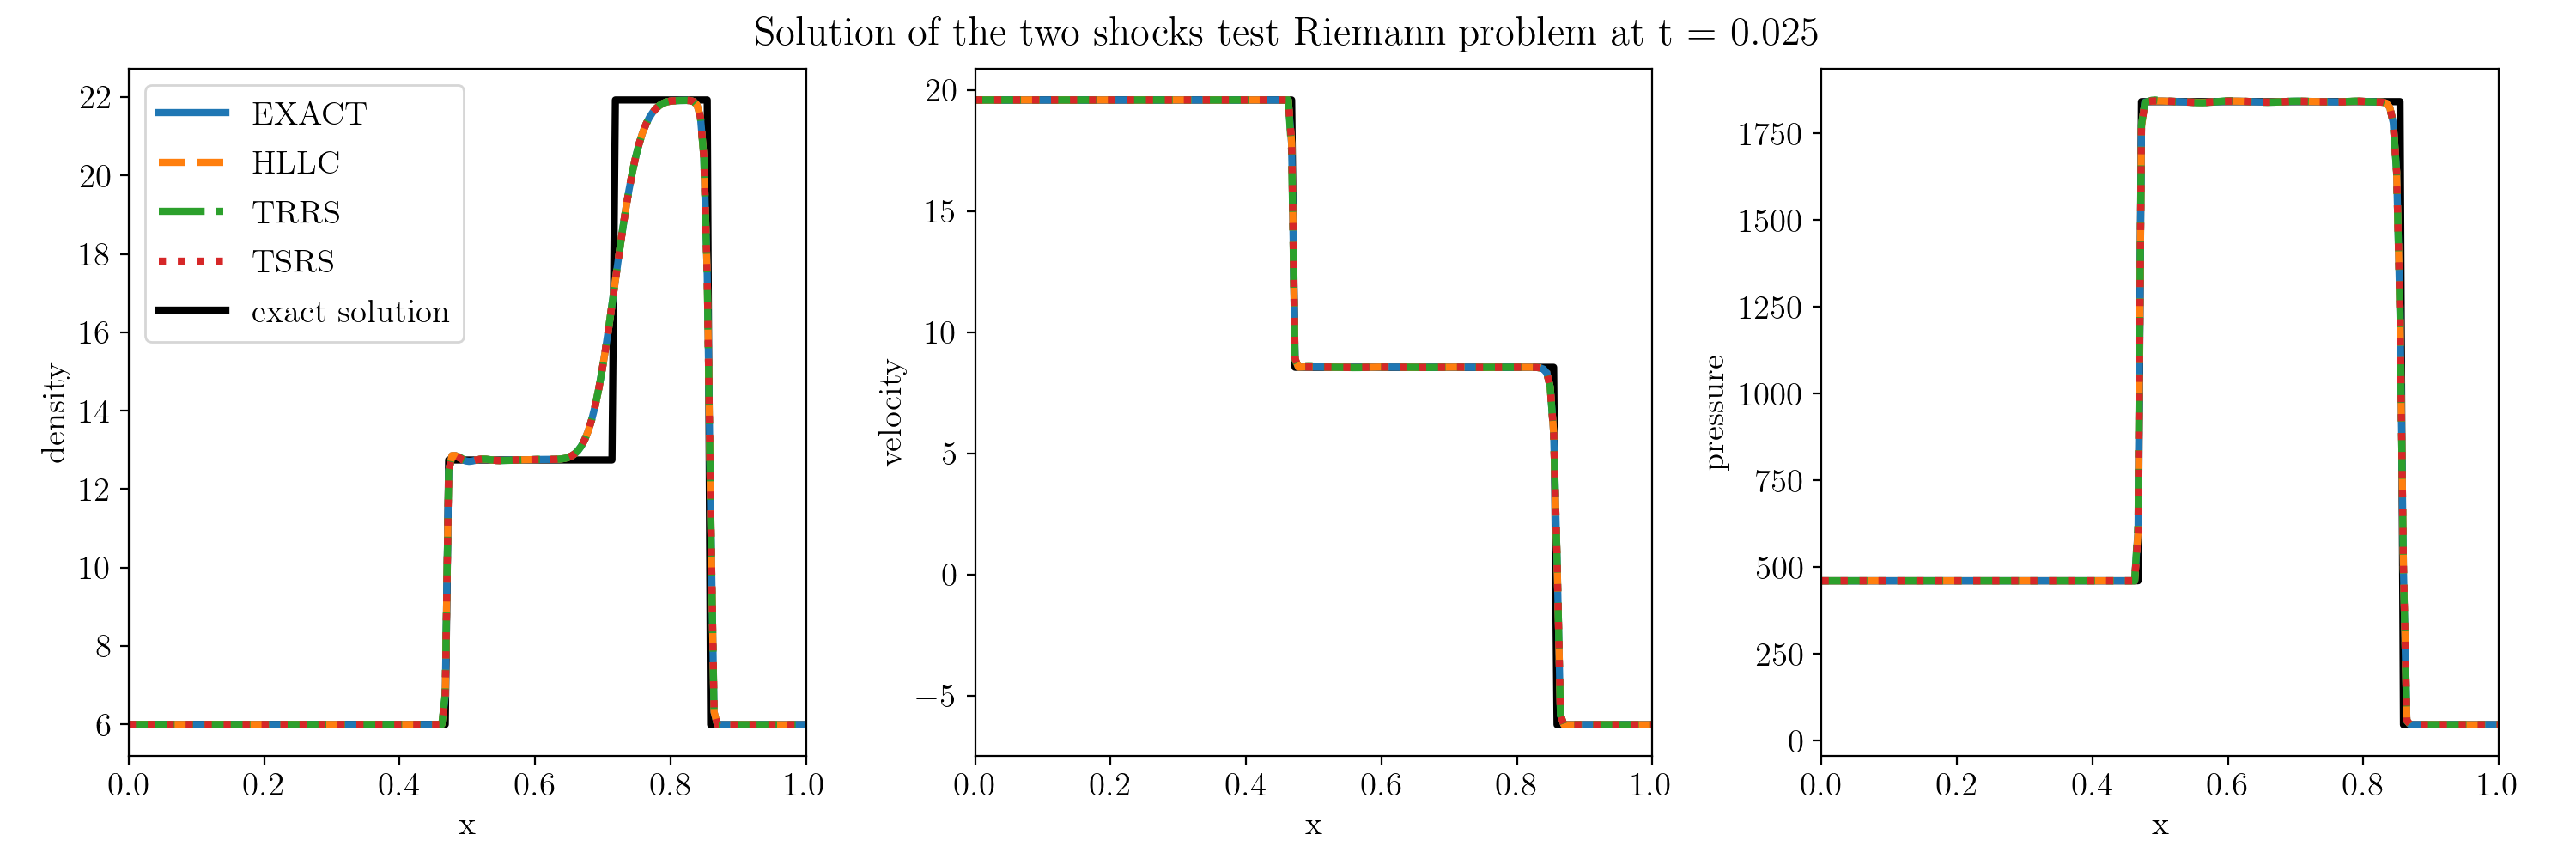
\includegraphics[width=\textwidth]{
    ./figures/FV/godunov_euler/GODUNOV-two_shocks-1D.png} %
    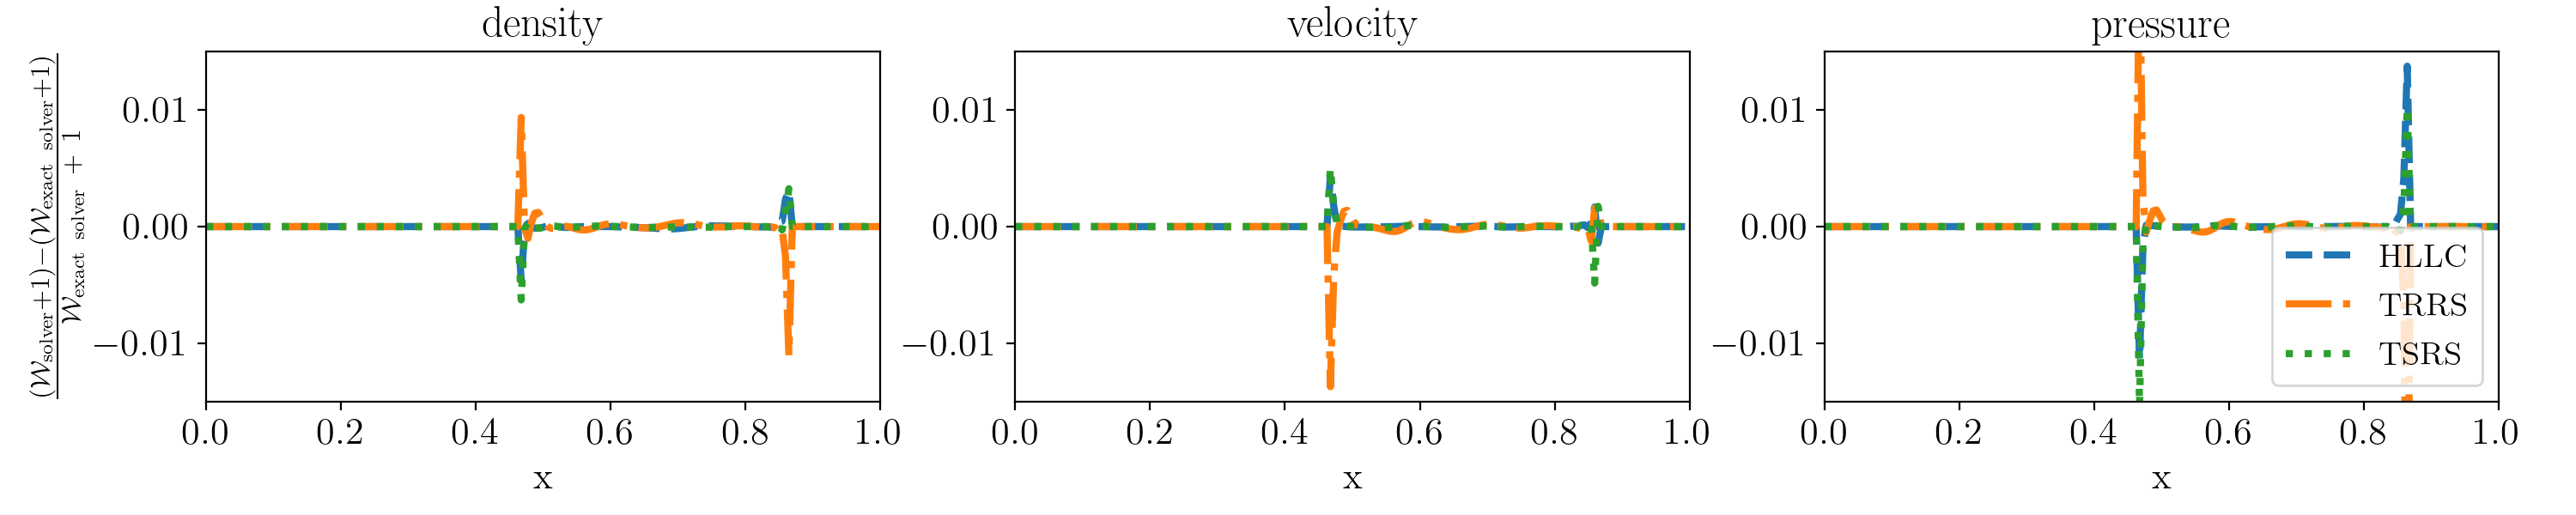
\includegraphics[width=\textwidth]{
    ./figures/FV/godunov_euler/GODUNOV-two_shocks-differences-1D.png} %
    \caption[Two shocks solution using Godunov's method]{
Top: The solution to the two shock test (eq. \ref{eq:two-shock-ICs}) using Godunov's method with
the exact, TRRS, TSRS, and HLLC Riemann solver, respectively, and the exact solution of the problem.
The exact solution consists of a two shocks on either side of the central contact wave. \\
Bottom: The relative differences of the solution of approximate Riemann solvers compared to the
solution using the exact Riemann solver with Godunov's method. The relative differences are
computed with all primitive quantities $\W = (\rho, v, p)$ being increased by 1 to avoid
divisions by zero.
    }%
    \label{fig:godunov-two-shocks}
\end{figure}





At this point, we're ready to put Godunov's method to use for the Euler equations. We can
make use of the fact that exact solutions to Riemann problems exist, and use them as a reference to
gauge the performance of the scheme. The results presented in what follows have been obtained using
the \meshhydro code.

Figure~\ref{fig:godunov-sod-test} shows the results of the ``Sod test'' Riemann problem with initial
conditions given in eq.~\ref{eq:sod-test-ICs}, where the exact solution consists of a left-facing
rarefaction and a right facing shock. Figure~\ref{fig:godunov-left-blast-wave} shows the results of
the so-called ``Left blast wave'' Riemann problem with initial conditions given in
eq.~\ref{eq:left-blast-wave-ICs}. The solution consists of a left-facing rarefaction and a right
facing shock. However in this test the shock is much stronger and much more prominent.
Figure~\ref{fig:godunov-two-shocks} shows the result of the ``two shock'' test with initial
conditions~\ref{eq:two-shock-ICs}. The solution consists of two shock waves, one on either side of
the central contact wave. In all three examples, the results using the exact Riemann solver as well
as the approximate TSRS, TRRS, and HLLC solvers are shown, along with relative differences of the
solutions obtained with approximate Riemann solvers compared to the solution obtained using the
exact Riemann solver in Godunov's method.

The choice of Riemann solver has negligible influence on the solution using Godunov's method,
affirming that the use of approximate solvers is an adequate approach. Aside from a few exceptions
around sharp discontinuities, the solutions with approximate Riemann solvers agree with the
solution using the exact Riemann solver to a level of below 1\%. In the presented tests, the
TRRS and the TSRS solver appear to perform better than the HLLC solver. This is however not
generally valid, and is due to the simple nature of the Riemann problem initial conditions that
have been used as the example test cases. The full solutions of the test problem consist of only
elementary waves, which the TRRS and TSRS solvers are able to handle rather well. In more complex
cases, the HLLC solver is may provide a better solution.

The method is able to successfully solve for the general structure of the exact solution, and all
emanating waves can be found. However, a noticeable feature is the lack of sharp discontinuities in
the solution using Godunov's method, where the exact solution should have some. Instead, Godunov's
method predicts smooth transitions. This is particularly noticeable for the density across contact
waves. The shock fronts aren't affected as much, but are nevertheless ``rounded off''.
On first sight, this may appear puzzling given that Godunov's method makes use of the integral form
of conservation laws, which explicitly allow for discontinuous solutions. So why doesn't it predict
solutions with sharp discontinuities? The answer is \emph{numerical diffusion}, which will be the
subject of the succeeding section.









%======================================================
\section{On Numerical Diffusion and Order Of Accuracy}\label{chap:numerical_diffusion}
%======================================================

%=============================================
\subsection{Numerical Diffusion}
%=============================================

To demonstrate and quantify the effect of numerical diffusion, let's apply Godunov's method to the
linear advection equation with constant coefficients, which greatly simplifies the required
computations.

The one dimensional linear advection equation with constant coefficients is given by

\begin{align}
    \deldt \uc + \deldx \fc = \deldt \uc + a \deldx \uc = 0, && a = \CONST
    \label{eq:numerical-diffusion-advection-equation}
\end{align}


The analytical solution is given by

\begin{align}
    \uc(x, t) = \uc(x - at, t=0)
\end{align}

which can be used to determine the solution of the Riemann problem with the initial left state
$\uc_L$ and right state $\uc_R$:

\begin{align}
    \uc(x, t>0) = \begin{cases}
                    \uc_L & \text{ if } x - at < 0 \\
                    \uc_R & \text{ if } x - at > 0
                  \end{cases}
\end{align}

Applied to the cell boundary $\uc_{i-\half}$ with initial left state $\uc_L = \uc_{i-1}$ and
right state $\uc_R = \uc_i$, and centering the problem at the boundary position $x_{i-\half}$,
the solution at the boundary is given by

\begin{align}
    \uc_{i-\half}(t>0) =
                \begin{cases}
                    \uc_{i-1} & \text{ if } - at < 0  \quad \Leftrightarrow \text{ if } a > 0  \\
                    \uc_{i} & \text{ if } - at > 0 \quad \Leftrightarrow \text{ if } a < 0
                \end{cases}
\end{align}

The solution for the right boundary is similarly given by

\begin{align}
    \uc_{i+\half}(t>0) =
                \begin{cases}
                    \uc_{i} & \text{ if } - at < 0  \quad \Leftrightarrow \text{ if } a > 0  \\
                    \uc_{i+1} & \text{ if } - at > 0 \quad \Leftrightarrow \text{ if } a < 0
                \end{cases}
\end{align}



In the interest of clarity, let's assume $a > 0$ in what follows.
Plugging the solution of the Riemann problem at the boundaries into definition into Godunov's
method, eq.~\ref{eq:godunov-scheme}, we get the expression

\begin{align}
    \uc_i^{n+1} = \uc_i^n + \frac{\Delta t}{\Delta x} a (\uc^{n}_{i-1} - \uc^{n}_{i})
\label{eq:godunov-advection}
\end{align}

The analytical solution for the linear advection equation with constant coefficients is
readily available, and dictates that the solution at any $t > 0$ should be just the initial state
$\uc (t = 0)$ translated to a new position $x' = x(t=0) + at$. This makes it easy to compare
the results obtained using Godunov's method to the exact solution of any initial conditions.
Figure~\ref{fig:linear-advection-godunov} shows the solution using Godunov's method for a step
function and a Gaussian at different times, moved back to the original position to demonstrate how
the initial shape changes over time. Evidently the same diffusive effects around discontinuities as
was the case for the Euler equations in
Figures~\ref{fig:godunov-sod-test}~-~\ref{fig:godunov-two-shocks} appear.


\begin{figure}
    \centering
    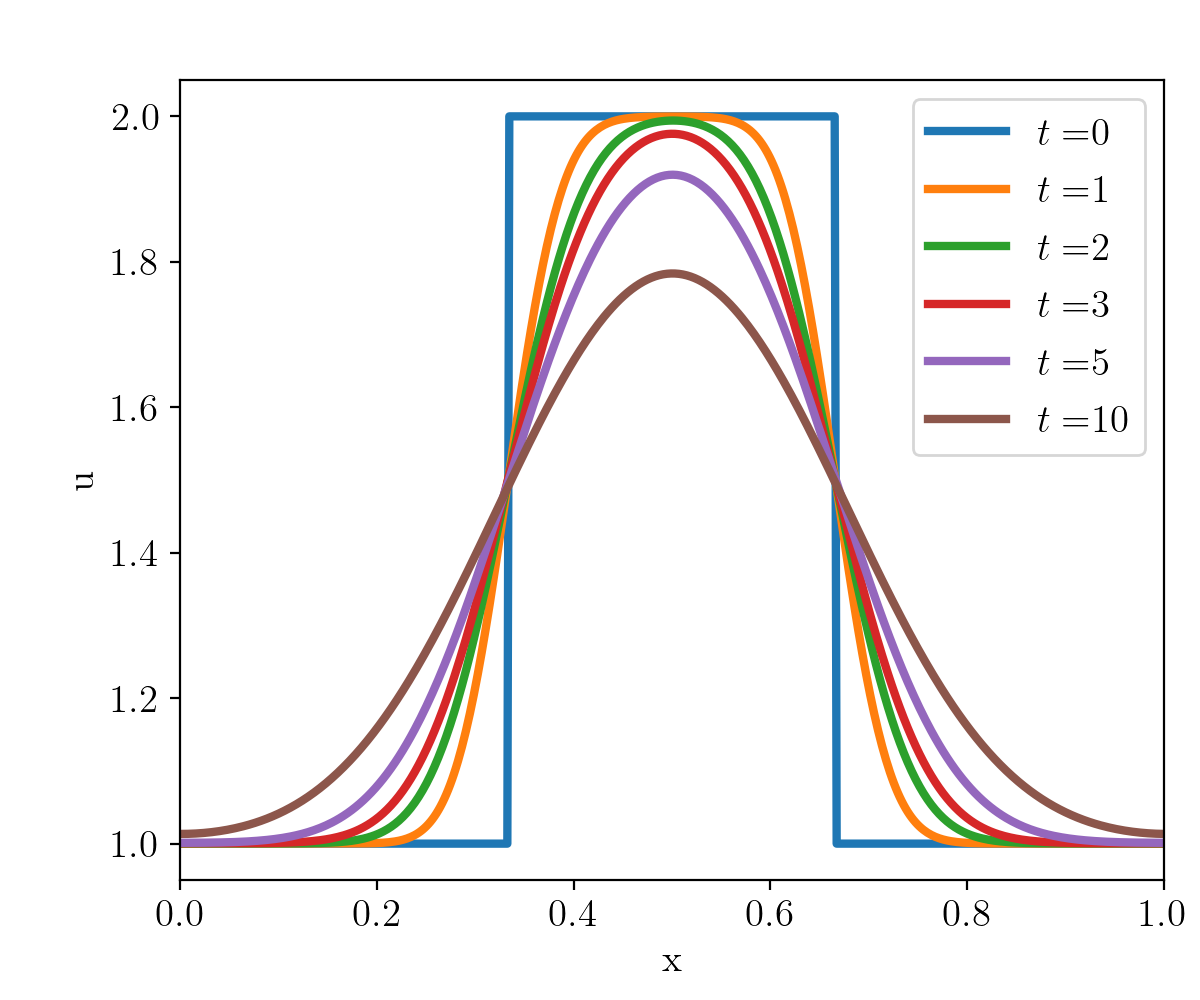
\includegraphics[width=.5\textwidth]{
    ./figures/FV/advection_pwconst/advection-1D-step.png}%
    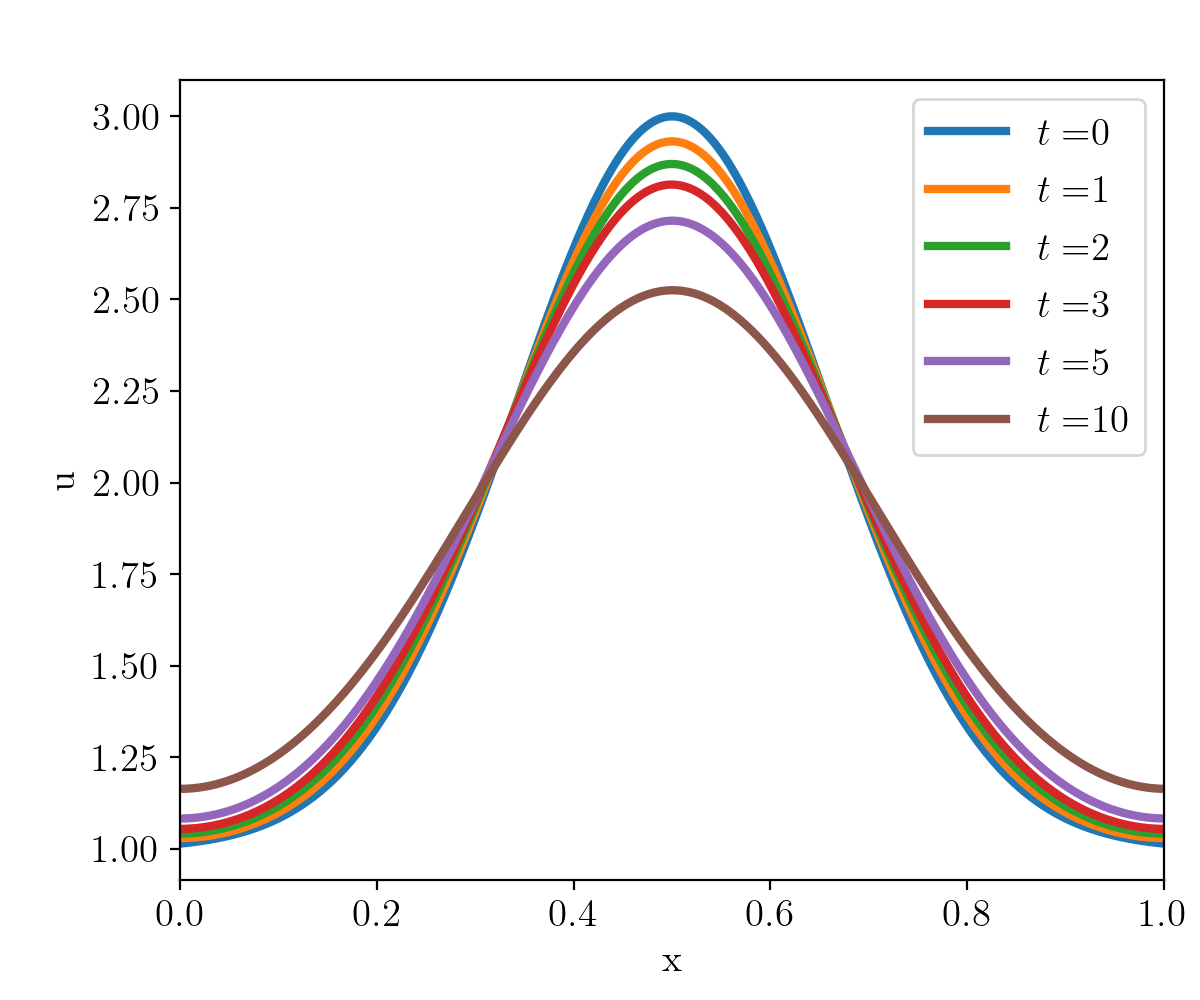
\includegraphics[width=.5\textwidth]{
    ./figures/FV/advection_pwconst/advection-1D-gaussian.png}%
    \caption[Linear advection with Godunov's method]{
The solution of the linear advection equation with constant coefficient $a = 1$ (in arbitrary
units). On the left, the initial conditions are a step function, on the right, they are a
Gaussian. The results at $t > 0$ have been repositioned to the original position to demonstrate
how the initial shape changes over time, which according to the analytical solution shouldn't
happen.
    }%
    \label{fig:linear-advection-godunov}
\end{figure}


To understand what is happening, we first take note of the fact that Godunov's scheme for linear
advection with constant coefficients is equivalent to a first order finite difference
discretization. Approximating

\begin{align}
    \deldt \uc &\approx \frac{\uc_i^{n+1} - \uc_i^n}{\Delta t} \\
    \deldx \fc &\approx \frac{\fc^{n}_{i} - \fc_{i-1}^n}{\Delta x}
        = a\frac{\uc^{n}_{i} - \uc_{i-1}^n}{\Delta x}
\end{align}

and plugging these approximations into the conservation
law~\ref{eq:numerical-diffusion-advection-equation} gives

\begin{align}
    \frac{\uc_i^{n+1} - \uc_i^n}{\Delta t} + a\frac{\uc^{n}_{i} - \uc_{i-1}^n}{\Delta x} = 0
    \label{eq:numerical-diffusion-finite-difference}
\end{align}

which is identical to Godunov's scheme~\ref{eq:godunov-advection}.

The terms $\uc_i^{n+1}$ and $\uc_{i-1}^n$ can be Taylor-expanded to second order in $\Delta t$ and
$\Delta x$:

\begin{align}
    \uc_i^{n+1} &=
        \uc_i^n + \Delta t \DELDT{\uc} +
        \frac{\Delta t^2}{2} \frac{\del^2 \uc}{\del t^2} + \mathcal{O}(\Delta t^3)
    \label{eq:taylor-un+1}\\
    \uc_{i-1}^{n} &=
        \uc_i^n - \Delta x \DELDX{\uc} +
        \frac{\Delta x^2}{2} \frac{\del^2 \uc}{\del x^2} + \mathcal{O}(\Delta x^3)
    \label{eq:taylor-ui-1}
\end{align}


Inserting these expansions into the discretized
equation~\ref{eq:numerical-diffusion-finite-difference} gives

\begin{align}
   & \frac{1}{\Delta t} \left[
        \uc_i^n + \Delta t \DELDT{\uc} +
        \frac{\Delta t^2}{2} \frac{\del^2 \uc}{\del t^2} + \mathcal{O}(\Delta t^3) - \uc_i^n
   \right] + \nonumber \\
   & \frac{a}{\Delta x} \left[
        \uc_i^n - \uc_i^n + \Delta x \DELDX{\uc} -
        \frac{\Delta x^2}{2} \frac{\del^2 \uc}{\del x^2} + \mathcal{O}(\Delta x^3)
   \right] = 0 \\
   = & \DELDT{\uc} + \frac{\Delta t}{2} \frac{\del^2 \uc}{\del t^2}
   + a \DELDX{\uc} - a \frac{\Delta x}{2} \frac{\del^2 \uc}{\del x^2}
    + \mathcal{O}(\Delta t^2) + \mathcal{O}(\Delta x^2)
\end{align}

keeping only the first order terms in $\Delta t$ and $\Delta x$, this can be rearranged to

\begin{align}
   \DELDT{\uc} + a \DELDX{\uc} =
   a \frac{\Delta x}{2} \frac{\del^2 \uc}{\del x^2}
   - \frac{\Delta t}{2} \frac{\del^2 \uc}{\del t^2} \label{eq:num-diff-intermediate}
\end{align}

The left hand side of eq.~\ref{eq:num-diff-intermediate} is identical to the conservation law we
are solving, and should be zero. Hence we can interpret everything on the right hand side as the
highest order error term that the numerical scheme introduces. Let's name it $Err$:

\begin{align}
    Err =
    a \frac{\Delta x}{2} \frac{\del^2 \uc}{\del x^2}
    - \frac{\Delta t}{2} \frac{\del^2 \uc}{\del t^2} \label{eq:num-diff-error}
\end{align}

To proceed, we express $\frac{\del^2 \uc}{\del t^2}$ as a function of $\frac{\del^2 \uc}{\del x^2}$
by differentiating the analytical advection equation once w.r.t. $t$:

\begin{align}
    \deldt \left( \deldt \uc + a \deldx \uc \right) =
    \frac{\del^2 \uc}{\del t^2} + a \frac{\del^2 \uc}{\del x \del t} = 0
\end{align}

and once w.r.t. $x$:
\begin{align}
    \deldx \left( \deldt \uc + a \deldx \uc \right) =
    \frac{\del^2 \uc}{\del x \del t} + a \frac{\del^2 \uc}{\del x^2} = 0
\end{align}

Relating these two derivatives over their common term $\frac{\del^2 \uc}{\del x \del t}$ gives us
the required relation:

\begin{align}
  -a \frac{\del^2 \uc}{\del x \del t}  =
      \frac{\del^2 \uc}{\del t^2} = a^2 \frac{\del^2 \uc}{\del x^2}
\end{align}

Which allows us to express the error $Err$ as

\begin{align}
    Err &=
    a \frac{\Delta x}{2} \frac{\del^2 \uc}{\del x^2}
    - \frac{\Delta t}{2} \frac{\del^2 \uc}{\del t^2}
    =
    a \frac{\Delta x}{2} \frac{\del^2 \uc}{\del x^2}
    + a^2 \frac{\Delta t}{2} \frac{\del^2 \uc}{\del x^2} \\
    &= \frac{a \Delta x}{2} \left( 1 - \frac{a \Delta t}{\Delta x} \right)
        \frac{\del^2 \uc}{\del x^2} \\
    &= \frac{a \Delta x}{2} \left( 1 - C_{CFL} \right)
        \frac{\del^2 \uc}{\del x^2}
\end{align}

Comparing this result and eqns.~\ref{eq:num-diff-intermediate} and \ref{eq:num-diff-error} with the
advection-diffusion equation\footnote{also called the ``convection-diffusion equation''}

\begin{align}
    \deldt \uc + a \deldx \uc = D \frac{\del^2 \uc}{\del x^2}  \label{eq:advection-diffusion}
\end{align}

it is clear that the error term that is introduced by the discretization of the equations is in
fact a diffusion term with the diffusion coefficient $D = \frac{a \Delta x}{2} \left( 1 - C_{CFL}
\right)$. This expression for $D$ also tells us how the diffusivity of the method will behave:

\begin{itemize}
 \item $D \propto \Delta x$: The diffusivity decreases with smaller grid spacing $\Delta x$
 \item $D \propto (1 - C_{CFL})$: The diffusivity decreases with bigger (maximal) time step sizes
    $C_{CFL}$.
\end{itemize}


\begin{figure}
    \centering
    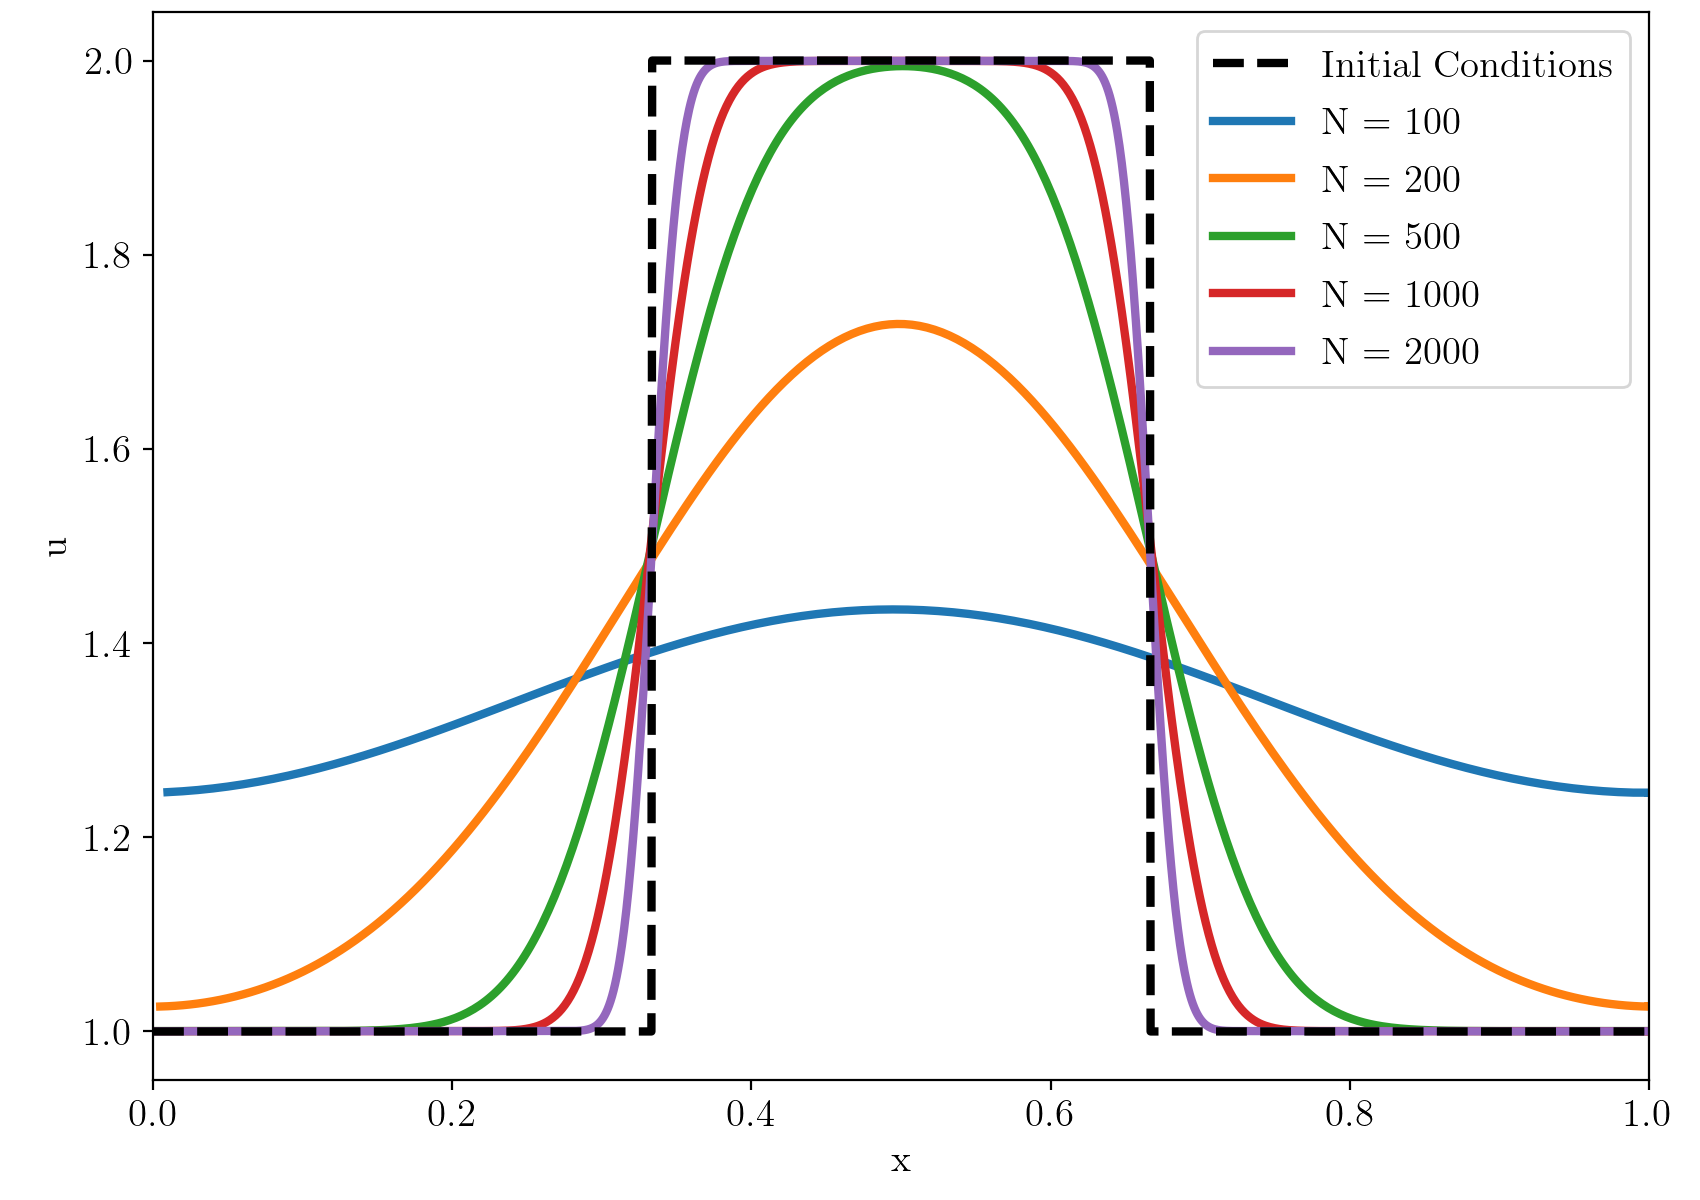
\includegraphics[width=.5\textwidth]{
    ./figures/FV/advection_pwconst/advection-1D-diffusivity-dx-step.png}%
    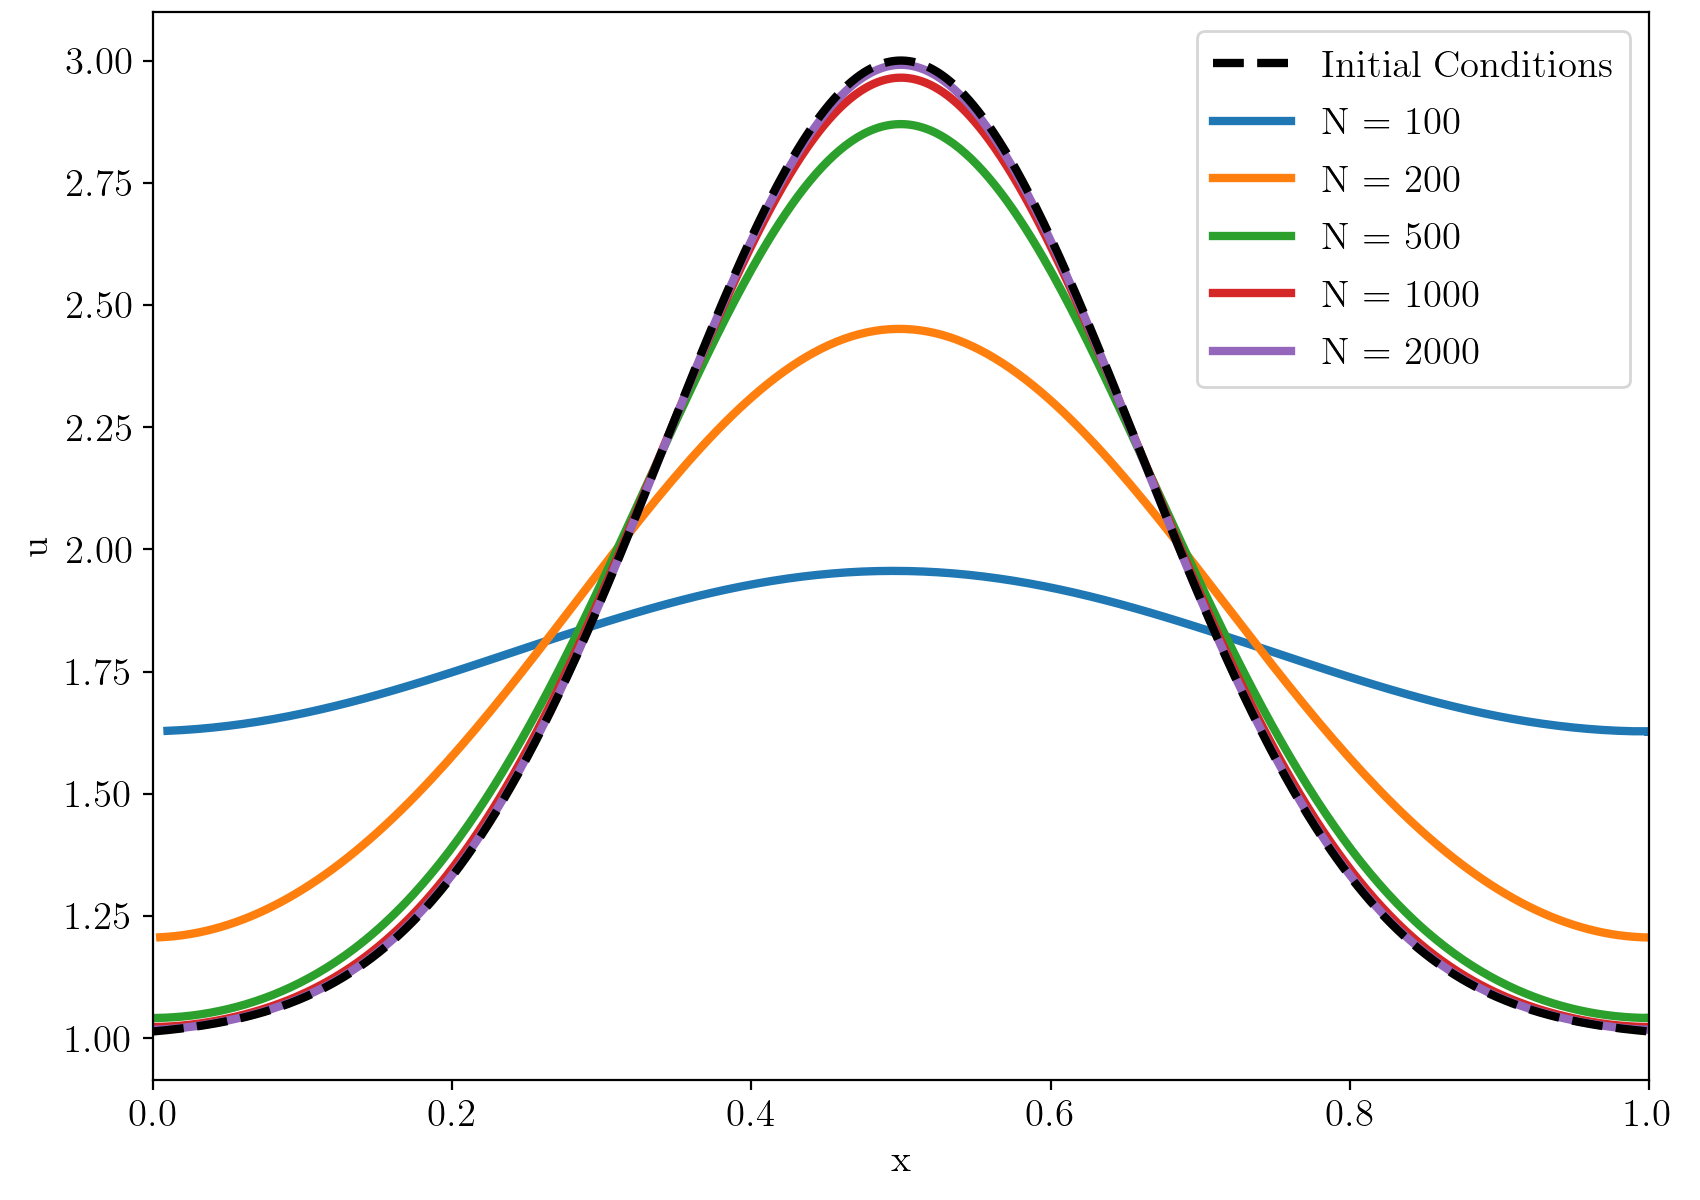
\includegraphics[width=.5\textwidth]{
    ./figures/FV/advection_pwconst/advection-1D-diffusivity-dx-gaussian.png}%
    \caption[Dependence of the numerical diffusion on $\Delta x$.]{
The solution of the linear advection equation with constant coefficient $a = 1$ (in arbitrary
units) for a fixed $C_{CFL} = 0.1$ and varying cell sizes $\Delta x = 1/N$ after $10^4$ time
steps. On the left, the initial conditions are a step function, on the right, they are a
Gaussian. The results have been repositioned to the original position at $t=0$ to demonstrate
how the initial shape changes over time.
}%
    \label{fig:linear-advection-diffusivity-dx}
\end{figure}


\begin{figure}
    \centering
    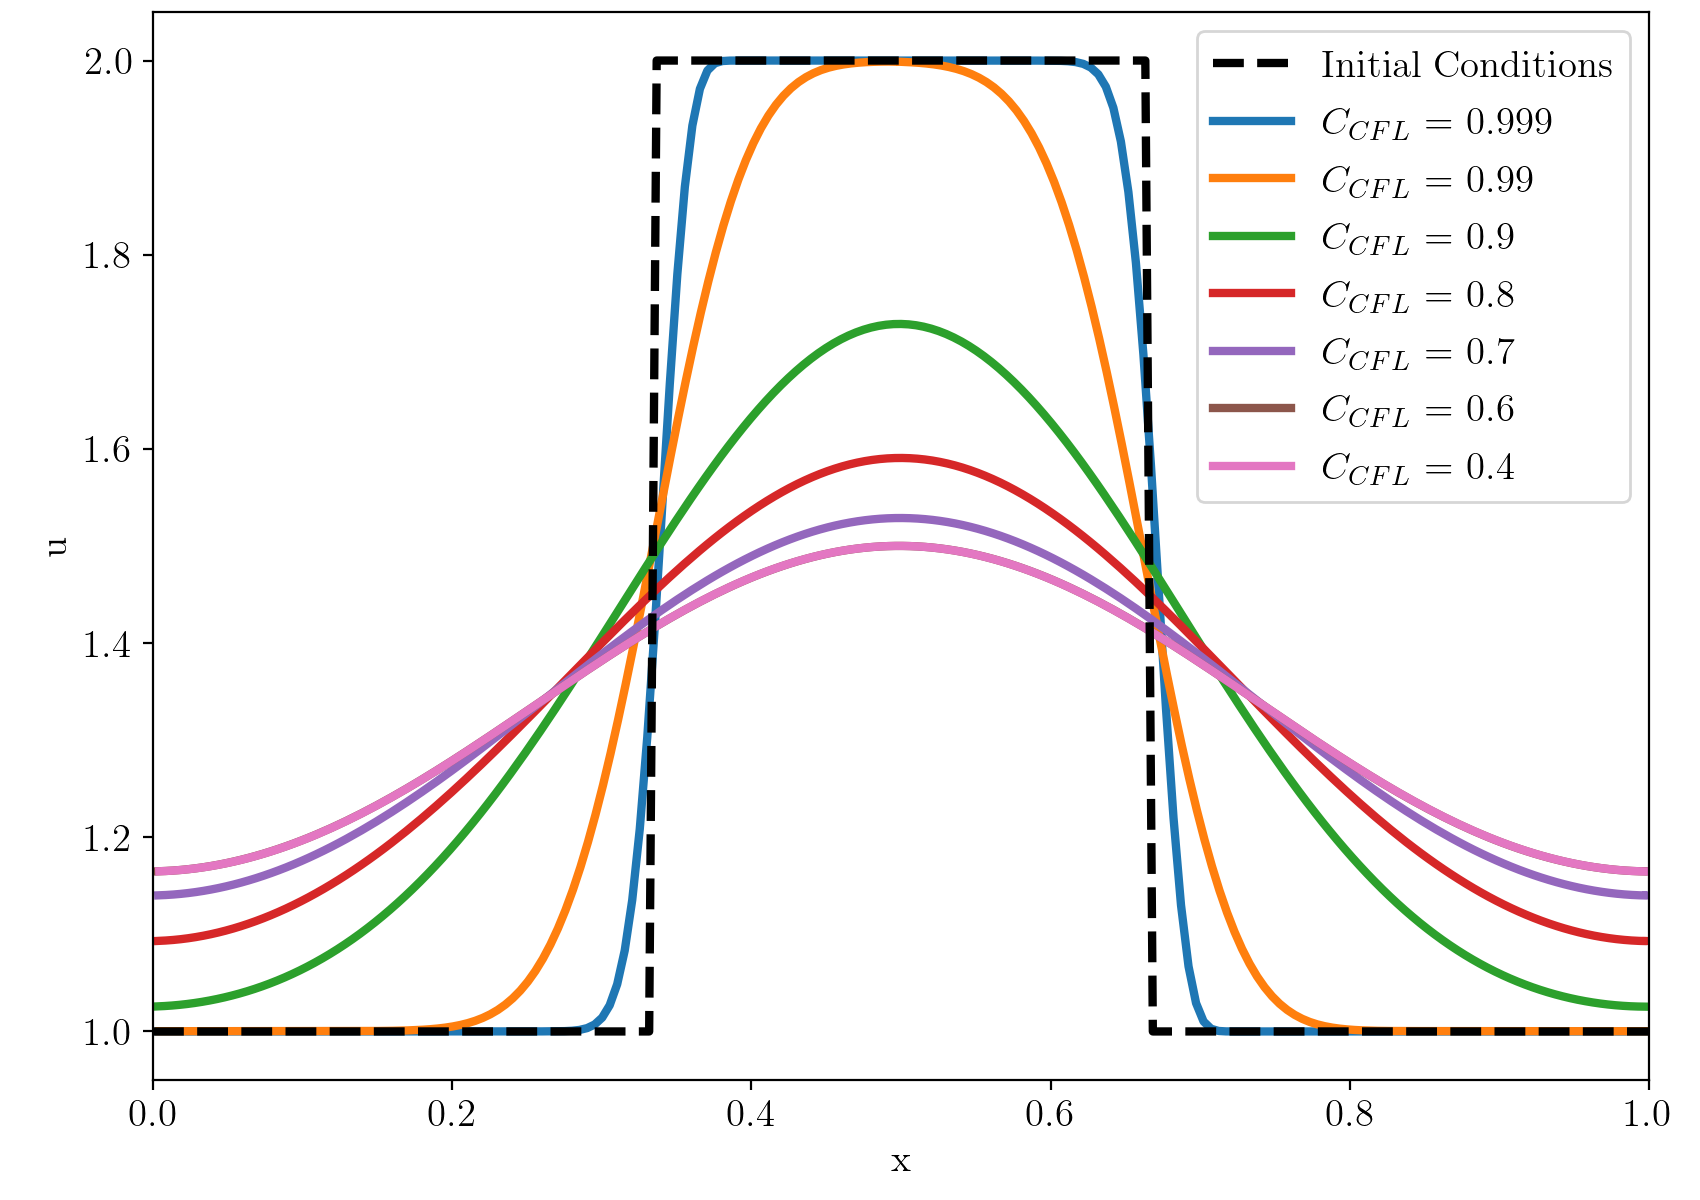
\includegraphics[width=.5\textwidth]{
    ./figures/FV/advection_pwconst/advection-1D-diffusivity-cfl-step.png}%
    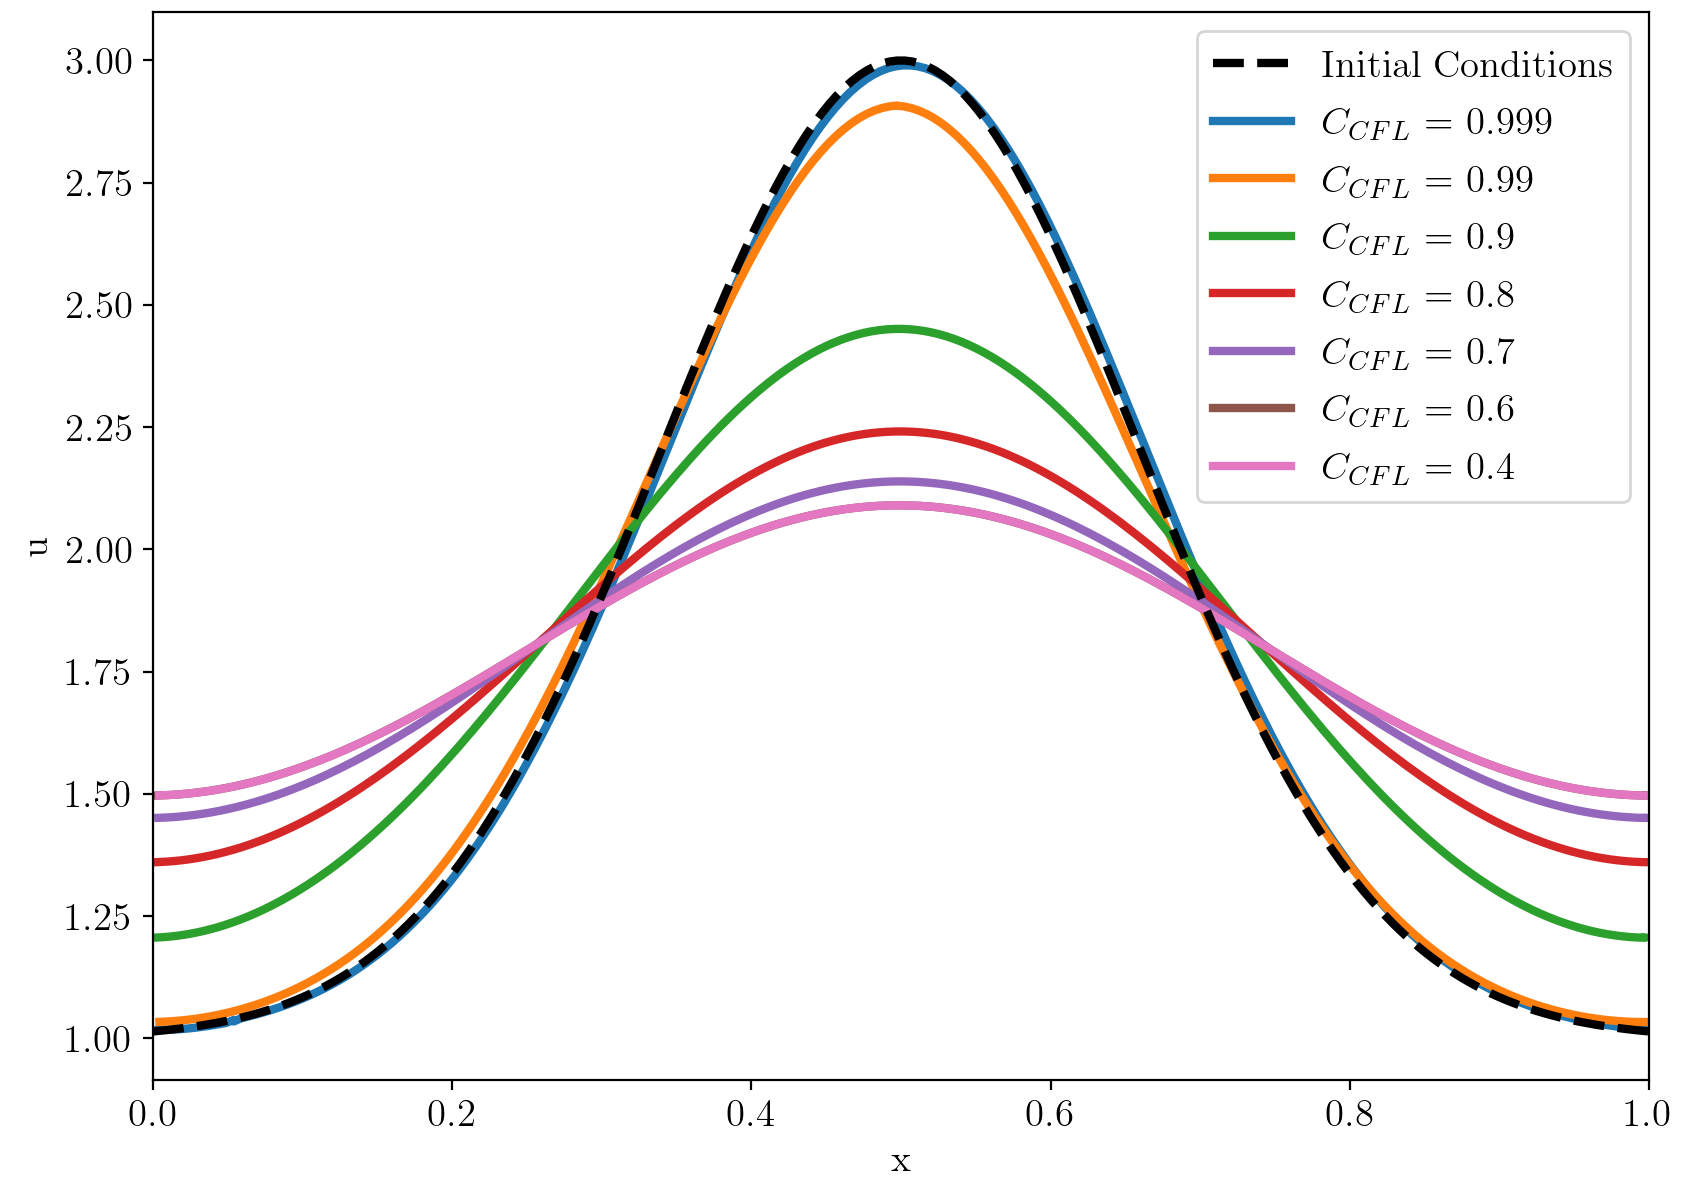
\includegraphics[width=.5\textwidth]{
    ./figures/FV/advection_pwconst/advection-1D-diffusivity-cfl-gaussian.png}%
    \caption[Dependence of the numerical diffusion on $C_{CFL}$.]{
The solution of the linear advection equation with constant coefficient $a = 1$ (in arbitrary units)
for fixed cell sized $\Delta x = 1/200$ and varying $C_{CFL}$ after $10^4$ time steps. On the left,
the initial conditions are a step function, on the right, they are a Gaussian. The results have been
repositioned to the original position at $t=0$ to demonstrate how the initial shape changes over
time.
    }%
    \label{fig:linear-advection-diffusivity-cfl}
\end{figure}


\begin{figure}
    \centering
    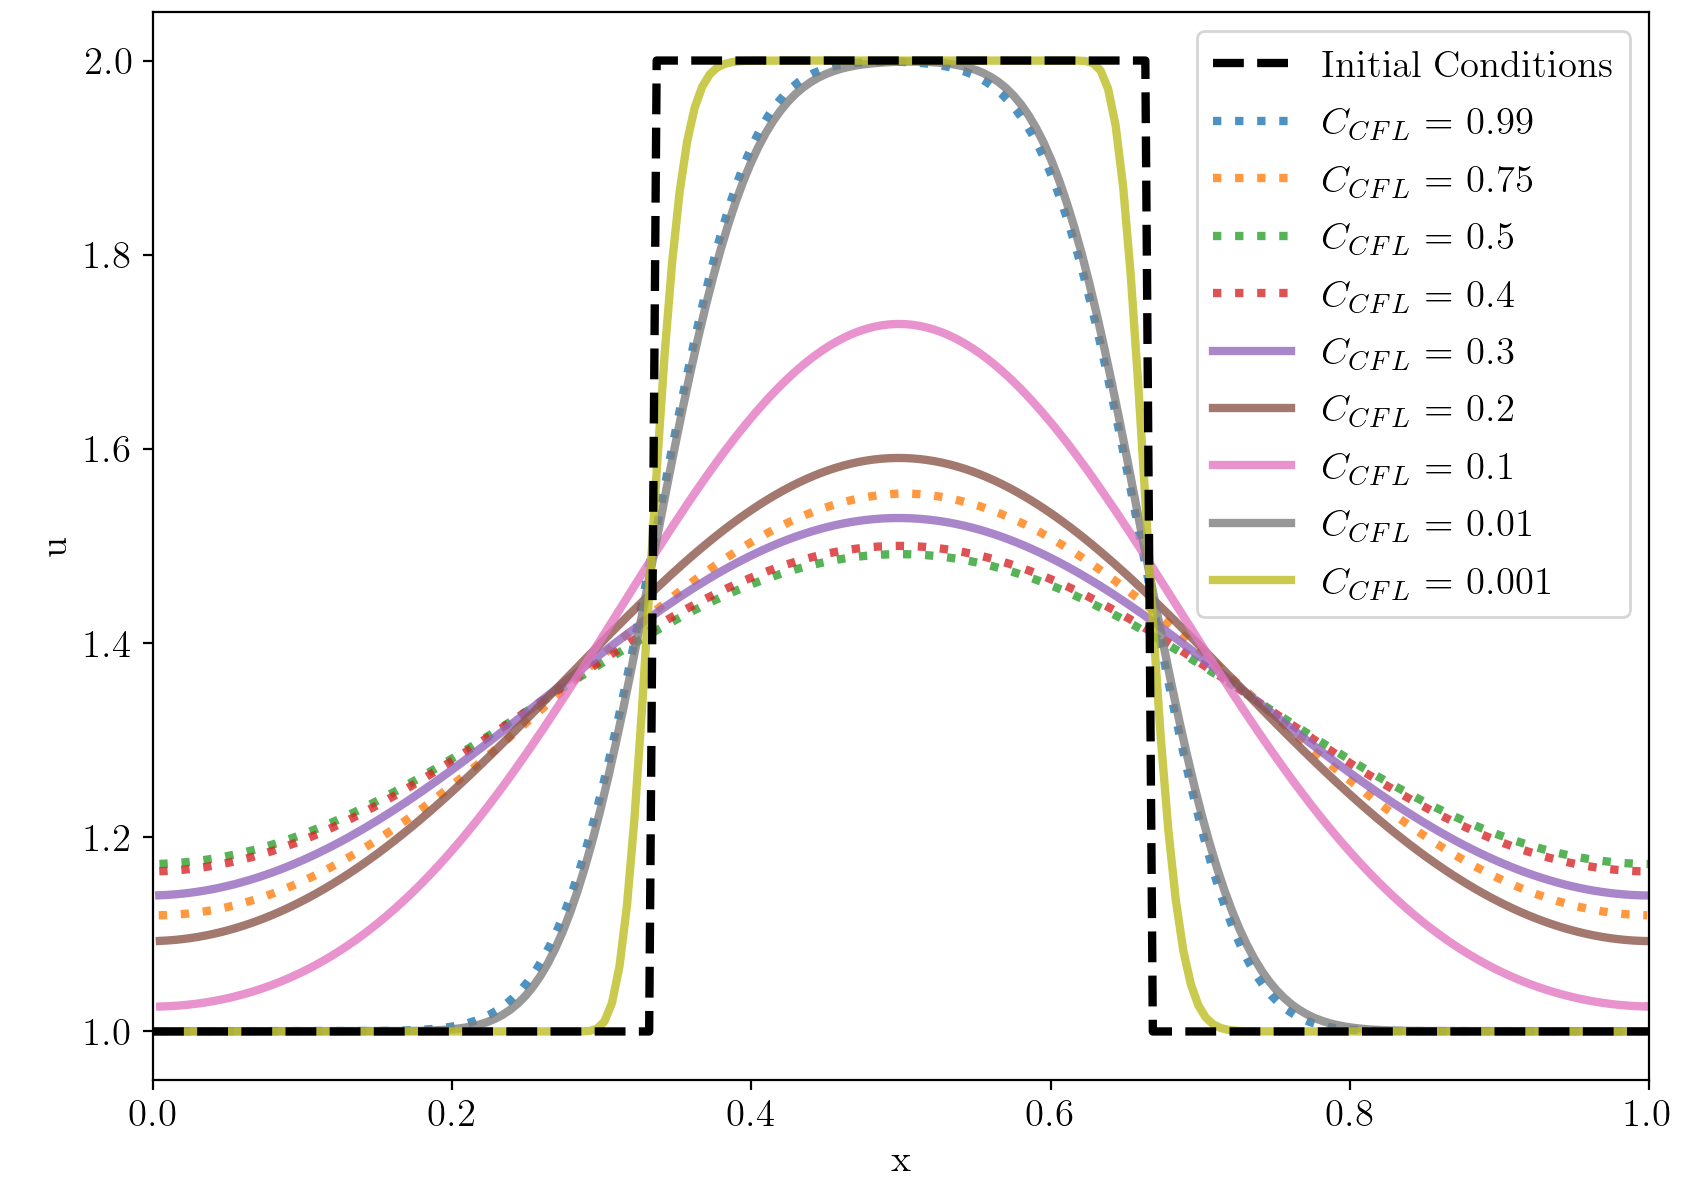
\includegraphics[width=.5\textwidth]{
    ./figures/FV/advection_pwconst/advection-1D-diffusivity-low-cfl-step.png}%
    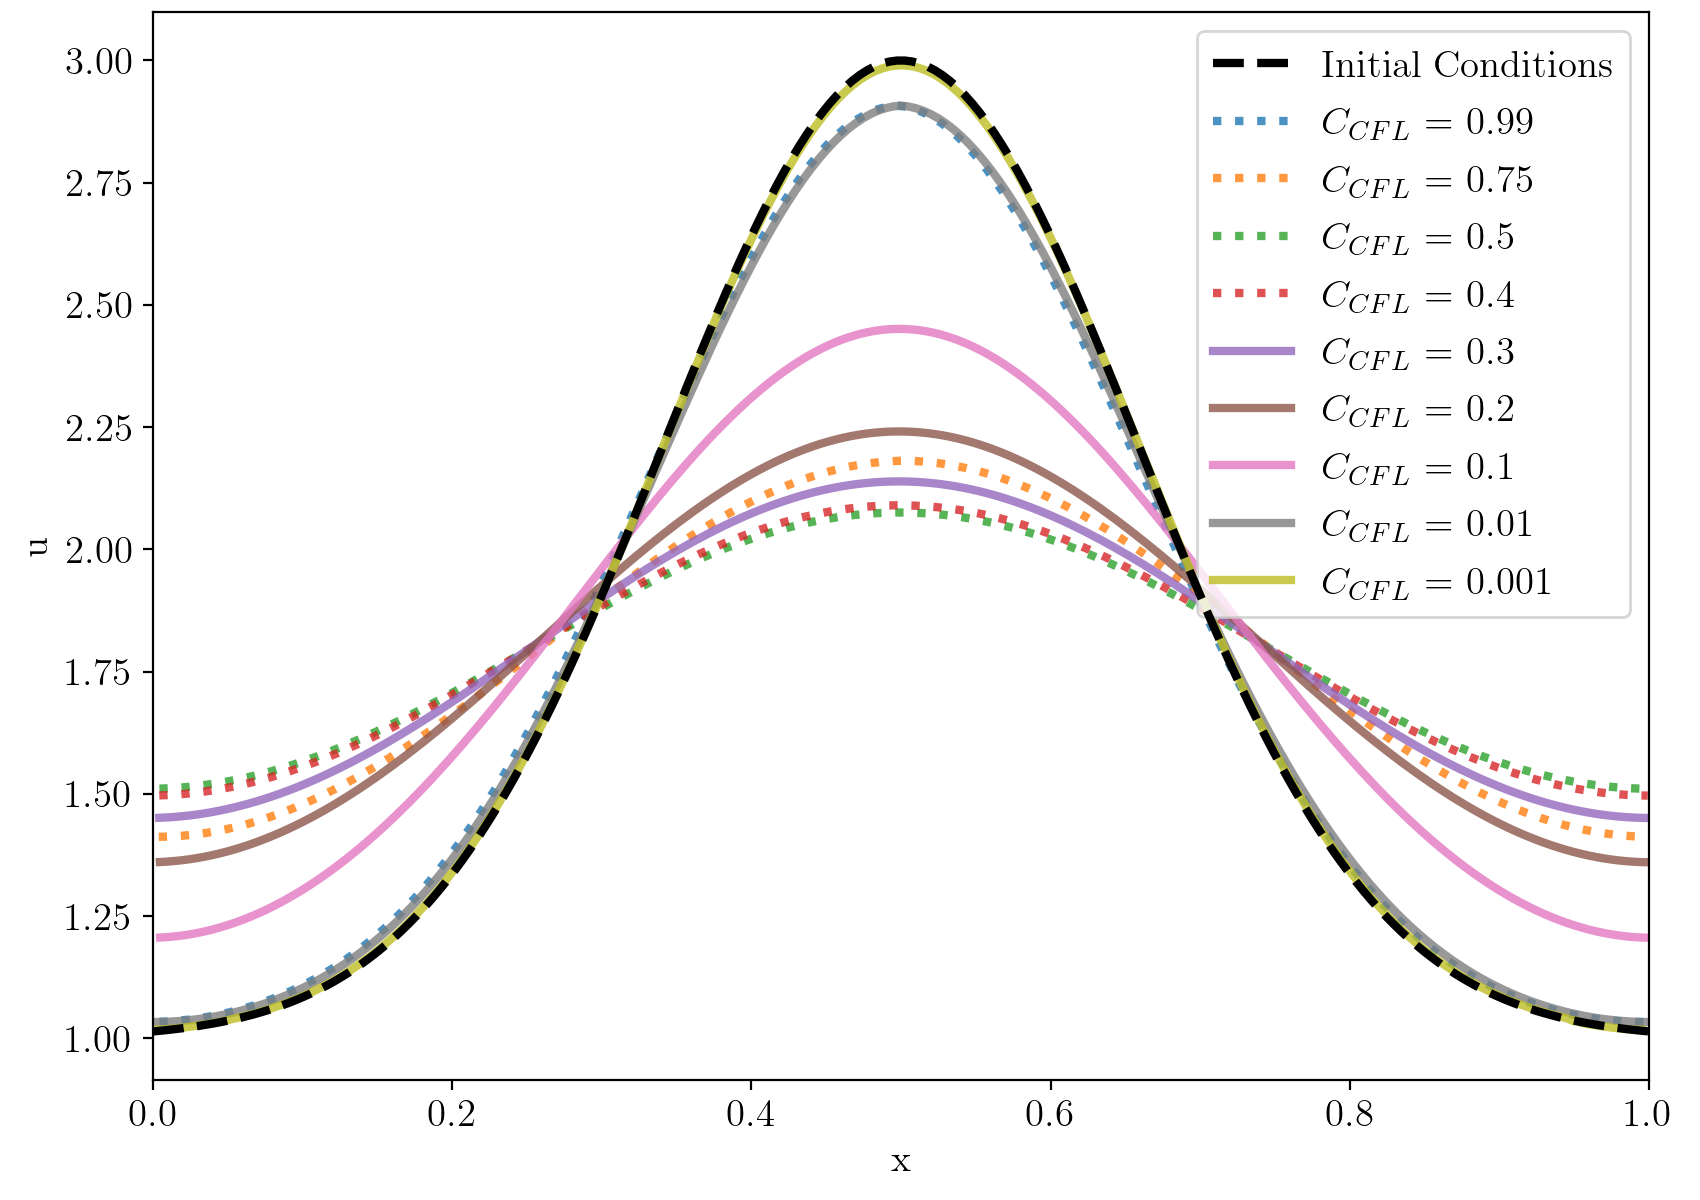
\includegraphics[width=.5\textwidth]{
    ./figures/FV/advection_pwconst/advection-1D-diffusivity-low-cfl-gaussian.png}%
    \caption[Dependence of the numerical diffusion on $C_{CFL}$ with very low $C_{CFL}$.]{
Same as Figure~\ref{fig:linear-advection-diffusivity-cfl}, but additionally going down to very low
$C_{CFL}$. At some point around $C_{CFL} \sim 0.5$, the solution begins to improve again.
    }%
    \label{fig:linear-advection-diffusivity-low-cfl}
\end{figure}


\begin{figure}
    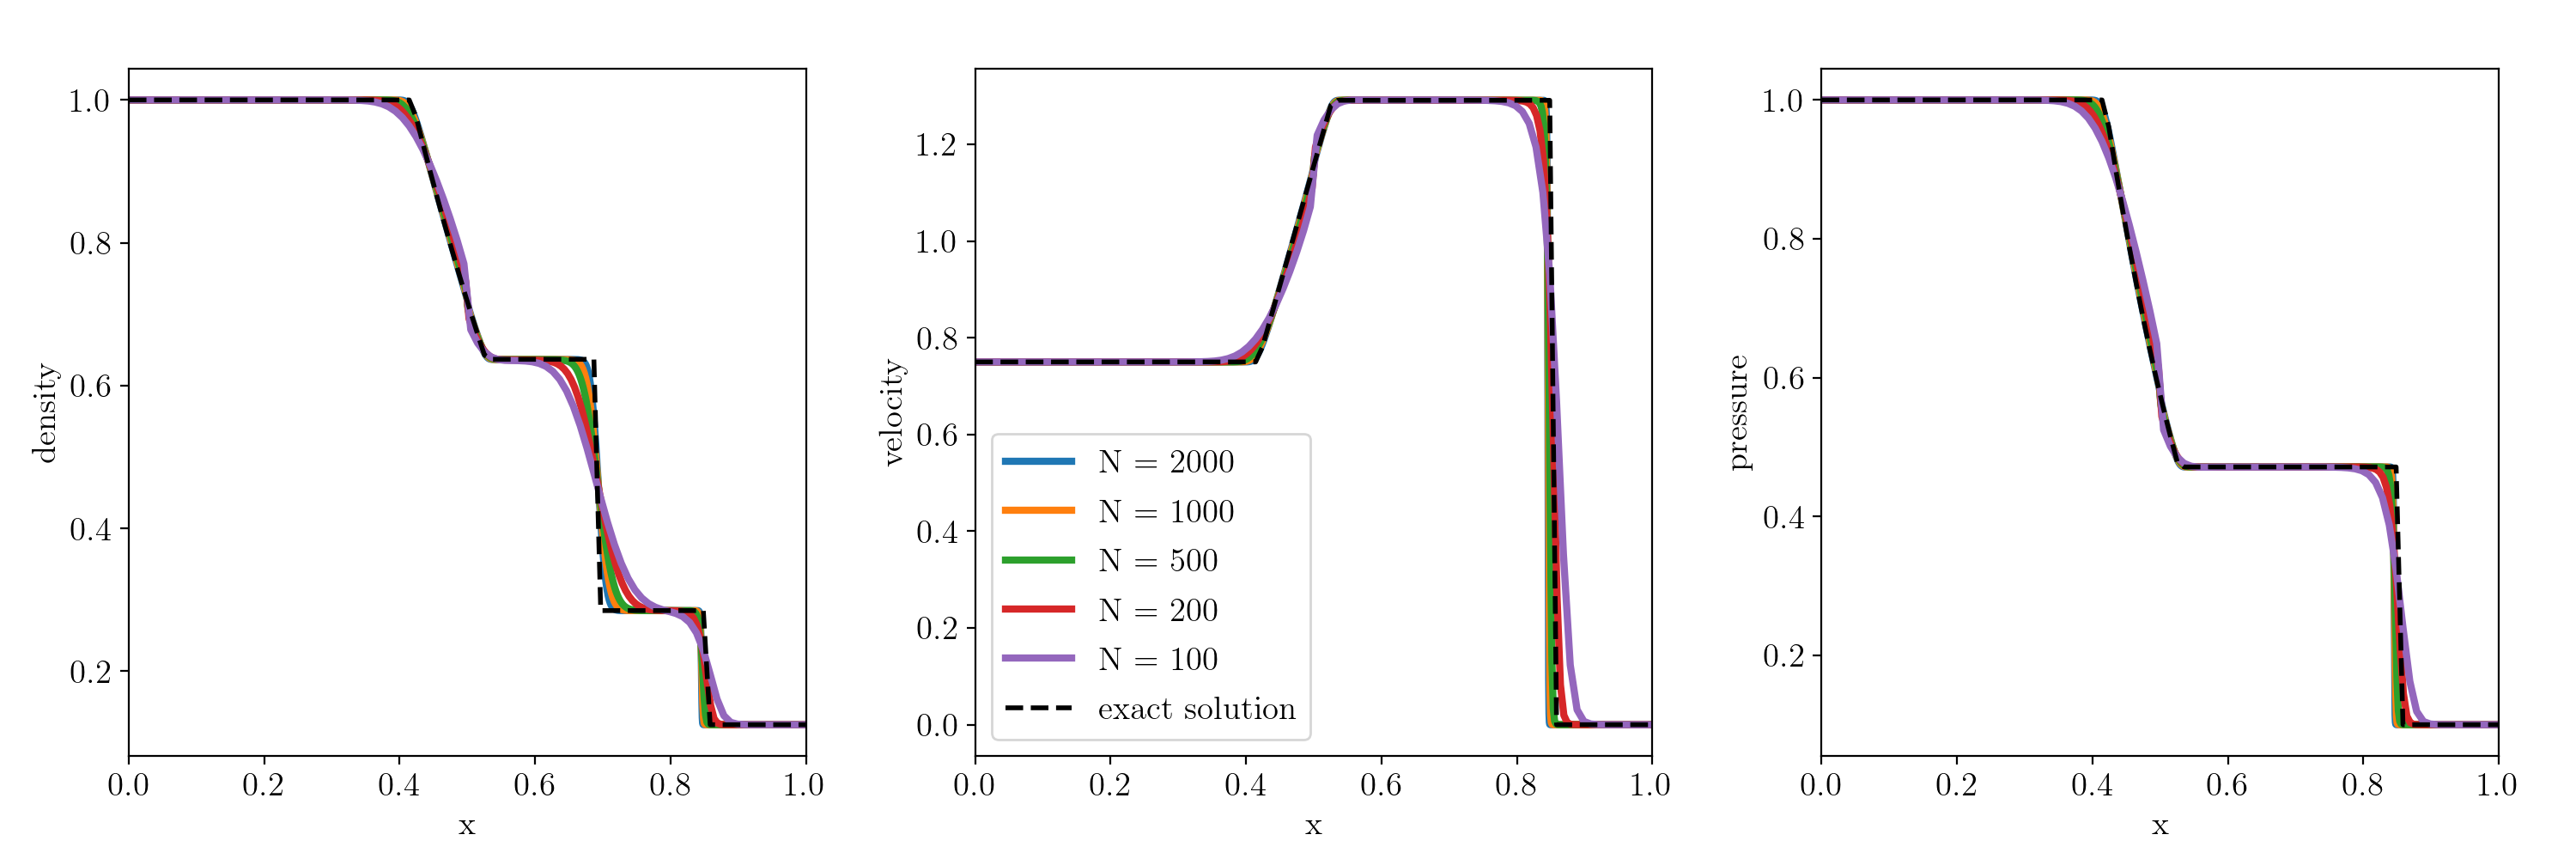
\includegraphics[width=\textwidth]{
    ./figures/FV/godunov_euler/godunov_euler_diffusivity-dx.png}%
    \caption[Dependence of the numerical diffusion on $\Delta x$ for the Sod test with
    Godunov's method]{
The Sod test problem (eq.~\ref{eq:sod-test-ICs}) for the Euler equations solved using varying
cell sizes $\Delta x = 1/N$ at time $t = 0.15$ (in arbitrary units).
    }%
    \label{fig:godunov-sod-test-diffusivity-dx}
\end{figure}






These findings can readily be tested, albeit with a caveat: The choices of $\Delta x$, $\Delta t$,
and $C_{CFL}$ are not independent. They are related through eq.~\ref{eq:godunov-cfl}, where in the
case of linear advection with constant coefficients $S_{max}^n = a$.
This means that if $C_{CFL}$ is kept fixed while $\Delta x$ is varied, the time step $\Delta t$ will
change as well. Naturally the same happens when $C_{CFL}$ is varied while $\Delta x$ is kept fixed.
If $\Delta x$ or $C_{CFL}$ decrease, the time step size $\Delta t$ decreases as well, meaning that
more time steps will be necessary to reach a given end time. The caveat here is that the total
error increases with the number of time steps, as deviations introduced each individual time step
accumulate. This can clearly be seen in Fig.~\ref{fig:linear-advection-godunov}, where $\Delta x$
and $C_{CFL}$ are constant, and the further the simulation progresses in time, the worse the
results become. So in order to obtain a meaningful and accurate comparison with respect to time
step size, we need to compare the results after a fixed number of time steps, and not at fixed
end times.

Figure~\ref{fig:linear-advection-diffusivity-dx} shows how the diffusivity decreases with decreasing
$\Delta x$, while Figure~\ref{fig:linear-advection-diffusivity-cfl} shows how the diffusivity
decreases as $C_{CFL}$ increases, confirming our previous findings. To confirm that the findings
also hold for Godunov's method applied to the Euler equations, the solution of the Sod test with
varying $\Delta x$ is shown in Figure~\ref{fig:godunov-sod-test-diffusivity-dx}.
However, for the sake of clarity the solutions here are shown for a fixed end time $t_{end} =
0.15$. While that is not ideal to showcase how the diffusivity behaves depending on $\Delta x$ and
$C_{CFL}$\footnote{
In fact, the accumulated error with the increased number of required time steps to get to a set
$t_{end}$ nearly exactly cancels out the variations when varying $C_{CFL}$, and all resulting
curves are nearly identical. For this reason, a figure containing how the diffusivity behaves  with
varying $C_{CFL}$ for Godunov's method for the Euler equations is omitted. Compare also to
Figure~\ref{fig:godunov-accuracy}.
}, the alternative where the total number of time steps is kept constant would
require to visualize solutions at different end times. Contrary to the solution of the linear
advection, the shape of the exact solution changes over time, so each result would take a different
shape, which leads to convoluted and unwieldy plots.









%=============================================
\subsection{Order of Accuracy}
%=============================================

An interesting thing occurs if we repeat the same experiment as in
Figure~\ref{fig:linear-advection-diffusivity-cfl}, but go down to even lower values of $C_{CFL}$.
The solution \emph{improves} again around $C_{CFL} \sim 0.5$, as is shown in
Figure~\ref{fig:linear-advection-diffusivity-low-cfl}. To understand this behavior, we need to look
into the order of accuracy of the scheme. To estimate the error introduced each step by the method,
which we call the one step error $Err_{OS}$, we compute the difference between the exact solution
$\uc_{i,e}^{n+1}$ at time $t^{n+1}$ and the predicted solution $\uc_i^{n+1}$ which is evaluated
using Godunov's method and exact initial conditions $\uc_i^n$:

\begin{align}
    Err_{OS}
    &= \uc_i^{n+1} - \uc_{i,e}^{n+1}  \\
    &= \uc_{e,i}^n - \frac{a \Delta t}{\Delta x} (\uc_{i,e}^n - \uc_{i-1,e}^n) - \uc_{i,e}^{n+1}
\end{align}

Using the Taylor expansions \ref{eq:taylor-un+1} and \ref{eq:taylor-ui-1} to express
$\uc_{i,e}^{n+1}$ and $\uc_{i-1,e}^n$, and keeping only second order terms in $\Delta x$ and
$\Delta t$, we can write

\begin{align}
    Err_{OS}
    &= \uc_{i,e}^n
        - a \frac{\Delta t}{\Delta x}
        \left( \uc_{i,e}^n -
            \uc_{i,e}^n +
            \DELDX{\uc_{i,e}^n } \Delta x -
            \frac{\Delta x^2}{2} \frac{\del ^2 \uc_{i,e}^n }{\del x^2}
            \order(\Delta x^3) \right)  - &&
\\
    &\quad  - \left(
        \uc_{i,e}^n +
        \DELDT{\uc_{i,e}^n } \Delta t +
        \frac{\Delta t^2}{2} \frac{\del ^2 \uc_{i,e}^n }{\del t^2}
        + \order(\Delta t^3)  \right) && \\
    &= - \Delta t \left(
        a \left(
            \DELDX{\uc_{i,e}^n } - \frac{\Delta x}{2} \frac{\del ^2 \uc_{i,e}^n }{\del x^2} +
\order(\Delta x^2)         \right)
        + \DELDT{\uc_{i,e}^n } + \frac{\Delta t}{2} \frac{\del ^2 \uc_{i,e}^n }{\del t^2} +
\order(\Delta t^2)
    \right) \\
    &= - \Delta t \left(
        \underbrace{\DELDT{\uc_{i,e}^n } + a\DELDX{\uc_{i,e}^n }}_{= 0} + \order(\Delta x) +
\order(\Delta t)
    \right)
\end{align}

Finally giving us:
\begin{align}
    Err_{OS} \propto \Delta t \left( \order(\Delta x) + \order(\Delta t) \right)
\label{eq:one-step-error}
\end{align}

While the one step error is proportional to $\Delta t^2$, reducing $\Delta t$ also means that more
steps need to be carried out to reach some end time $t_{end}$. If for some initially set $\Delta
t_0$ one needs $N$ steps to reach $t_{end}$, i.e. $t_{end} = N \Delta t_0$, then for some $\Delta
t_1 < \Delta t_0$ we require $t_{end} = N (\Delta t_0 / \Delta t_1)$ steps. It is then convenient to
define the Local Truncation Error $Err_{LT}$

\begin{align}
    Err_{LT} = \frac{1}{\Delta t} Err_{OS}
\end{align}

to describe how a scheme scales with cell spacing $\Delta x$ and time step size $\Delta t$. For
this scheme,

\begin{align}
    Err_{LT} = \order(\Delta t) + \order(\Delta x) \label{eq:local_truncation_error}
\end{align}

so Godunov's scheme is first order accurate in $\Delta x$ and $\Delta t$.

This property explains why in Figure~\ref{fig:linear-advection-diffusivity-low-cfl} the results
begin to improve once $C_{CFL}$ becomes small enough. The diffusion term $D \propto (1 - C_{CFL})$
has an upper boundary at $C_{CFL} = 0$. Once $C_{CFL}$ is small enough, the diffusion term stops
increasing noticeably. For example, going from $C_{CFL} = 0.01$ to $C_{CFL} = 0.001$ changes the
amplitude of the diffusion term form $0.99$ to $0.999$, or less than one per cent. However, since
the Courant number directly determines the time step size $\Delta t$ and the scheme is first order
accurate in time, the expected result when going from $C_{CFL} = 0.01$ to $C_{CFL} = 0.001$ should
improve by a factor of 10. In the case of the solution of the linear advection equation using
Godunov's method, the turnaround point, where the results begin to improve again, occurs at
$C_{CFL} \sim 0.5$ (see Figure~\ref{fig:linear-advection-diffusivity-low-cfl}).

Another interesting point can be made when comparing the results for the step function with the
results of the smooth Gaussian: It appears that the deviations from the expected solution for the
step function are somewhat larger, in particular in cases with lower diffusivity, i.e. for small
$\Delta x$ in Figure~\ref{fig:linear-advection-diffusivity-dx} and large $C_{CFL}$ in
Figure~\ref{fig:linear-advection-diffusivity-cfl}.

To understand that phenomenon, we need to look into a different approach to estimate the local
truncation error using a formalism that allows for discontinuous solutions. The previous expression
assumed a smooth (differentiable) state, which is not the case any longer with discontinuities
being present. Instead, we make use of the analytical solution for the advection-diffusion
equation~\ref{eq:advection-diffusion} as the analytical expression for the solution Godunov's
scheme will provide. This solution is given by

\begin{align}
    \uc^n(x) = \uc_0(x - a t^n) \ \mathrm{erfc}\left(\frac{x - at^n}{\sqrt{4 D t}} \right)
\end{align}

with

\begin{align}
    \mathrm{erfc}(x) = \frac{2}{\sqrt{\pi}} \int_x^\infty \exp (-z^2) \de z
\end{align}


To estimate the error at time $t^n$, we take the 1-norm of the difference between the exact
solution $\uc_e = \uc_0{x - at^n}$ and the analytical expression of the solution of Godunov's
scheme:

\begin{align}
    Err &= || \uc_e(x, t^n) - \uc^n(x) ||_1
        = \int\limits_{-\infty}^{\infty} | \uc_e(x, t^n) - \uc^n(x) | \de x \\
        &= \int\limits_{-\infty}^{\infty}
            | \uc_0(x - at) - \uc_0(x - at) \ \mathrm{erfc}\left(\frac{x - at^n}{\sqrt{4 D t}}
\right)) | \de x \\
        &= \int\limits_{-\infty}^{\infty}
            | \uc_0(x') (1 - \mathrm{erfc}\left(\frac{x'}{\sqrt{4 D t}} \right)) | \de x'
\end{align}

In the last step, the substitution $x' = x - at$ was used. Choosing the discontinuous initial
conditions

\begin{align}
    \uc_0 = \begin{cases}
            1 & \text{ if } x < 0\\
            0 & \text{ if } x > 0\\
            \end{cases}
\end{align}

and using a second substitution $y = \frac{-x'}{\sqrt{4 D t}}$ the integral can be written as

\begin{align}
    Err &= \int\limits_{-\infty}^{0}
        | (1 - \mathrm{erfc}\left(\frac{x'}{\sqrt{4 D t}} \right)) | \de x' \\
        &= \sqrt{4 D t} \int\limits^{\infty}_{0}
        | (1 - \mathrm{erfc}(-y)) | \de y
\end{align}

The integral can be further simplified, but since it will in any case yield a result independent of
$x$ and $t$, we don't actually care for its exact evaluation, and instead write

\begin{align}
    Err = C_1 \sqrt{D t} = C_2 \sqrt{\Delta x t} = C_2 \sqrt{\Delta x N \Delta t}
\label{eq:error-discontinuity}
\end{align}

where $C_1$ and $C_2$ are some constants independent of $\Delta x$ and $\Delta t$. Note that in
order to derive this result, we chose the initial conditions to be discontinuous. So this
result tells us that in the presence of discontinuities, the error scales with $\sqrt{\Delta t}$ and
$\sqrt{\Delta x}$, while for smooth conditions, it scales with $\Delta t$ and $\Delta x$. The exact
factor of $\sqrt{\Delta t}$ and $\sqrt{\Delta x}$ difference to the smooth condition isn't
generally valid for other methods and initial conditions, but it is a fact that the presence of
discontinuities reduces the order of accuracy of a scheme just like it did in this case.


Finally, to conclude the chapter on Godunov's method, we can verify our findings of the order of
accuracy of the method by conducting numerical experiments and measuring how the error scales with
$\Delta x$ and $C_{CFL} \propto \Delta t$. The error is estimated using

\begin{align}
    Err = \frac{1}{N} \sum_i^N |\uc_i - \uc_{i,exact}|
\end{align}


Figure~\ref{fig:linear-advection-accuracy} shows the results for the linear advection equation with
constant coefficients using Godunov's method. Both a step function containing discontinuities and
smooth Gaussian initial conditions are used. Also results for both a fixed number of time steps and
for a fixed end time are shown, along with guiding lines for varying powers of $\Delta x$. Let's
look at the results of each of the four cases:

\begin{itemize}
\item For the smooth Gaussian and a fixed number of total time steps (blue dashed line), the error
scales with $\sim \Delta x^2$. The reason is that for a fixed $C_{CFL}$, reducing $\Delta x$
also reduces the time step $\Delta t$. We have seen that the local truncation
error~\ref{eq:local_truncation_error} depends on both $\Delta t$ and $\Delta x$, and in this
scenario, \emph{both} are reduced, leading to a net scaling with a power greater than $1$. Another
way of understanding this phenomenon is by considering the fact that the one step
error~\ref{eq:one-step-error} is proportional to $\Delta t^2$. By keeping the total number of time
steps fixed for all $\Delta x$, the amount of errors that can be accumulated over the course of the
simulation is kept constant, resulting in a scaling $\propto \Delta t^2 = (C_{CFL} \Delta x / a)^2
\propto \Delta x^2$ for constant $a$ and $C_{CFL}$.

\item For the smooth Gaussian and a fixed end time $t_{end} = 2$ (blue solid line), the error
scales with $\sim \Delta x$, which is exactly what the local truncation
error~\ref{eq:local_truncation_error} predicts. In this scenario, the accumulation of individual
one step errors due to the larger number of total time steps necessary with decreasing $\Delta x$
reduces the total accuracy. However, this line is the one that is of higher interest for practical
applications: After all, typically a simulation is run until a specified end time, not for a
certain number of steps.

\item The discontinuous step function and a fixed end time $t_{end} = 2$ (orange solid line), the
error is as predicted by eq.~\ref{eq:error-discontinuity}: Since the end time $t_{end} = N \Delta
t$ is kept constant, the result should be precisely an error $\propto \sqrt{\Delta x}$.

\item The discontinuous step function and a fixed total number of steps time (orange dashed line),
the error scales with $\sim \Delta x$, which is again higher than for the case with a fixed end
time. The reason is that since the end time is not being kept constant, the factor $\sqrt{N \Delta
t}$ is not constant any more. $N$ is constant, but $\Delta t \propto \Delta x$ for a fixed
$C_{CFL}$, and the error scales in total $\propto \sqrt{\Delta x \Delta x} = \Delta x$, which is
exactly what we observe.
\end{itemize}


The case for varying $C_{CFL}$ and fixed $\Delta x$ in Figure~\ref{fig:linear-advection-accuracy}
is somewhat simpler to interpret, since the choice of $C_{CFL}$ doesn't affect the cell spacing
$\Delta x$. For a fixed number of time steps, the expected slopes $\propto C_{CFL}$ and $\propto
C_{CFL}^{1/2}$ for the smooth and the discontinuous, respectively, are reproduced. In the cases for
a fixed end time, the accumulation of one step errors cancels out the improved accuracy per step,
and the net scaling is $\propto 1$. In all cases, the influence of the diffusion term $D \propto (1
- C_{CFL})$ is clearly seen for $C_{CFL} \gtrsim 0.1$. The same behavior can be seen for Godunov's
method applied to the Euler equations in Figure~\ref{fig:godunov-accuracy}, since the solved
problem, the Sod test (eq.~\ref{eq:sod-test-ICs}), contains discontinuities as part of its exact
solution.



\begin{figure}
    \centering
    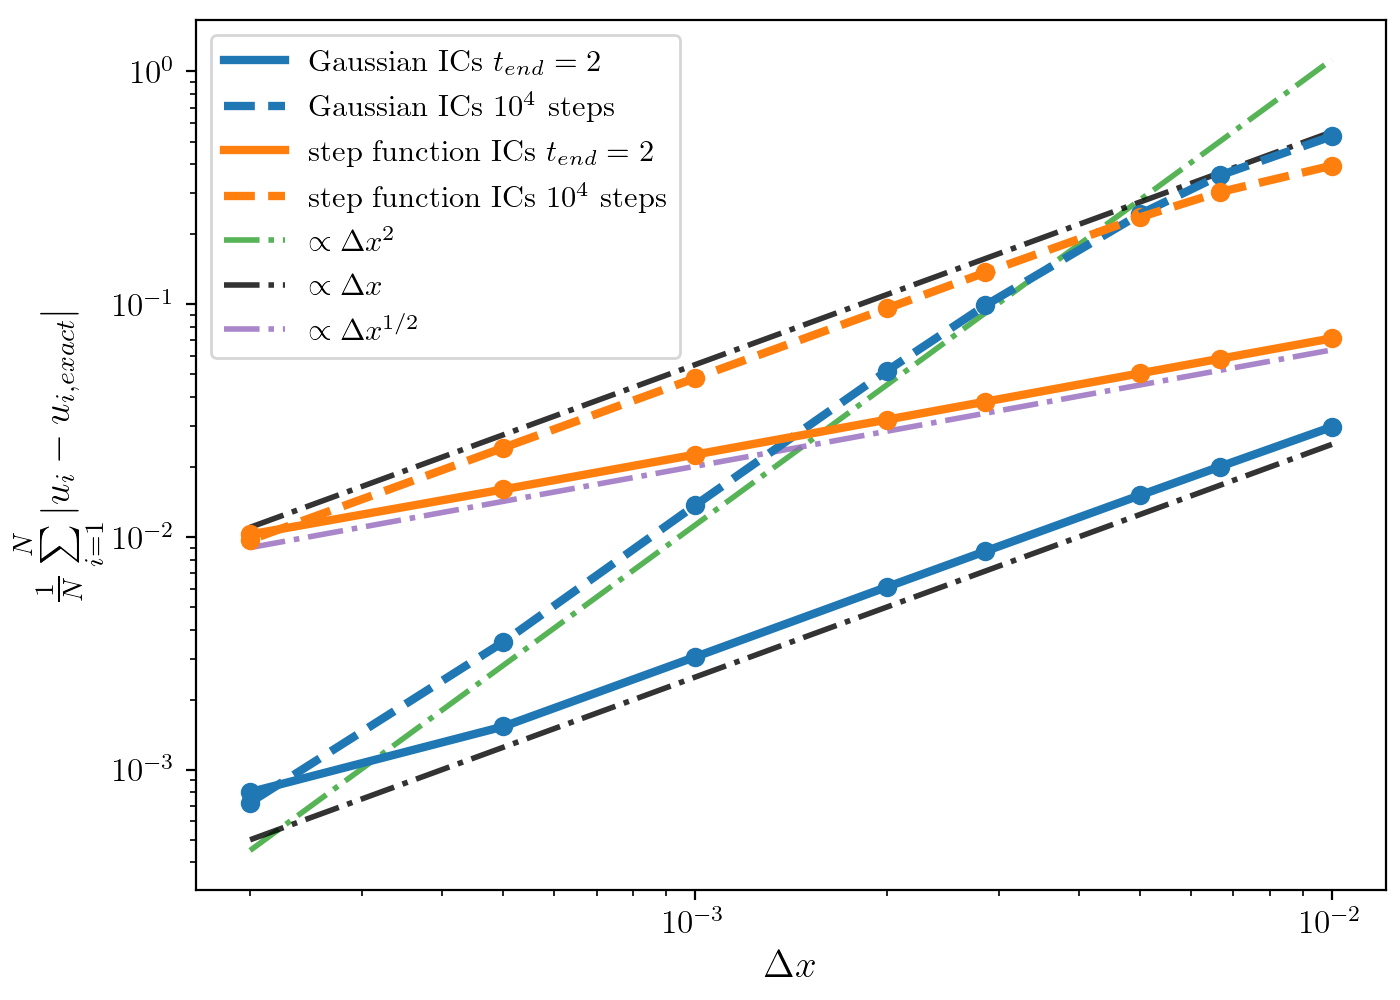
\includegraphics[width=.5\textwidth]{
    ./figures/FV/advection_pwconst/accuracy_dx.png}%
    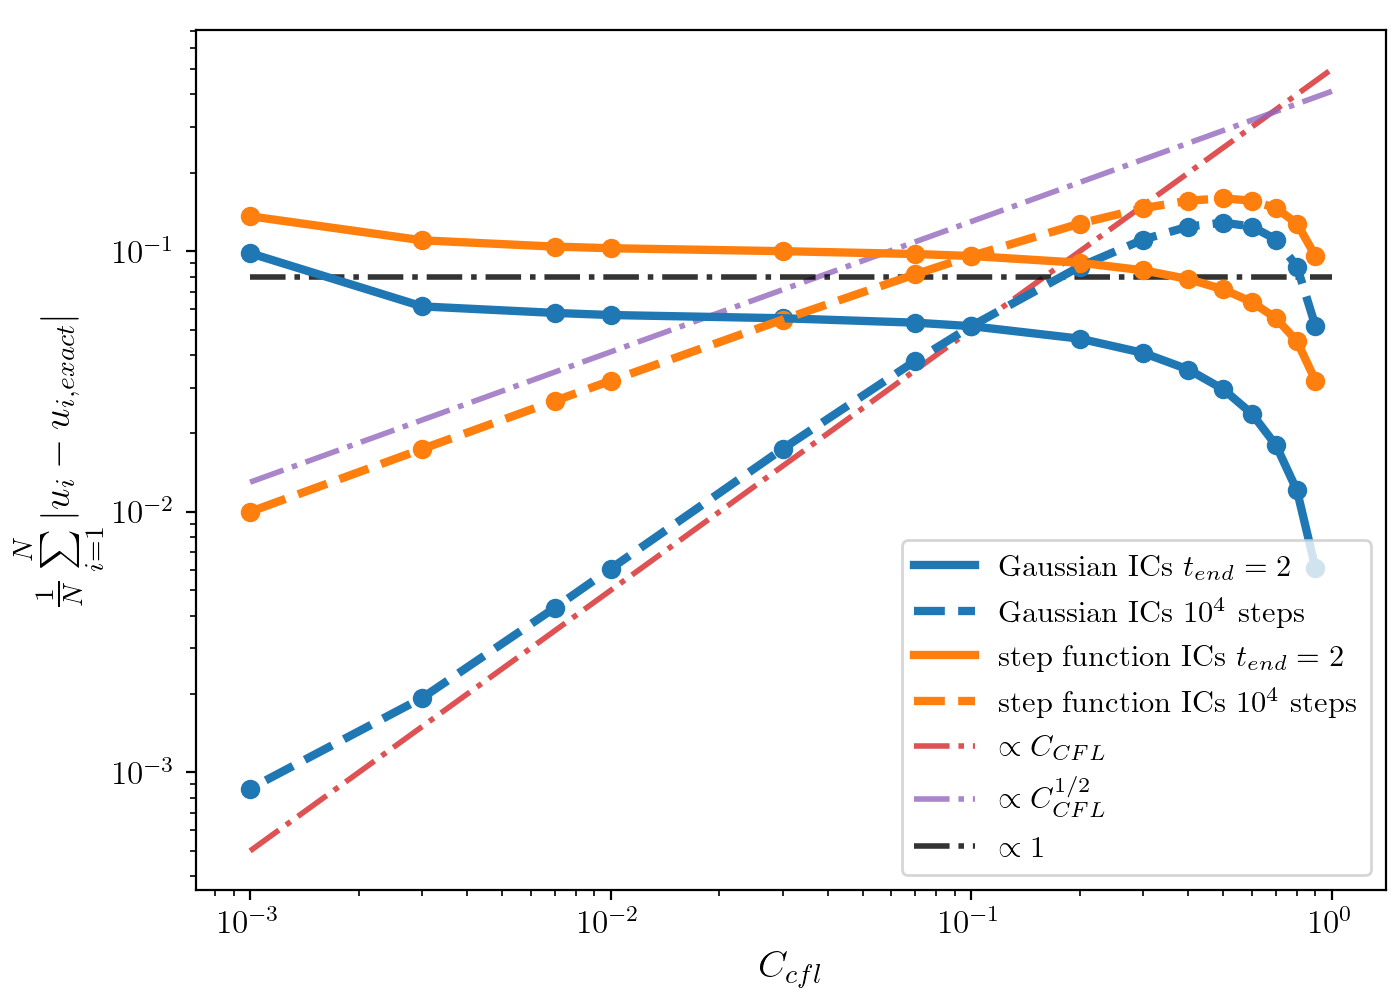
\includegraphics[width=.5\textwidth]{
    ./figures/FV/advection_pwconst/accuracy_CFL.png}%
    \caption[Order of accuracy w.r.t $\Delta x$ and $C_{CFL}$ for linear advection using Godunov's
method.]{
The order of accuracy w.r.t. $\Delta x$ (left) and the Courant number $C_{CFL}$ (right) of
the linear advection equation with constant coefficients using Godunov's method for both a step
function and a Gaussian initial conditions. For comparison, lines with slopes $1/2$, $1$, and $2$
are overplotted. The experiments are run for both a fixed end time $t_{end} = 2$ as well as for a
fixed total number of time steps individually.
    }%
    \label{fig:linear-advection-accuracy}
\end{figure}





\begin{figure}
    \centering
    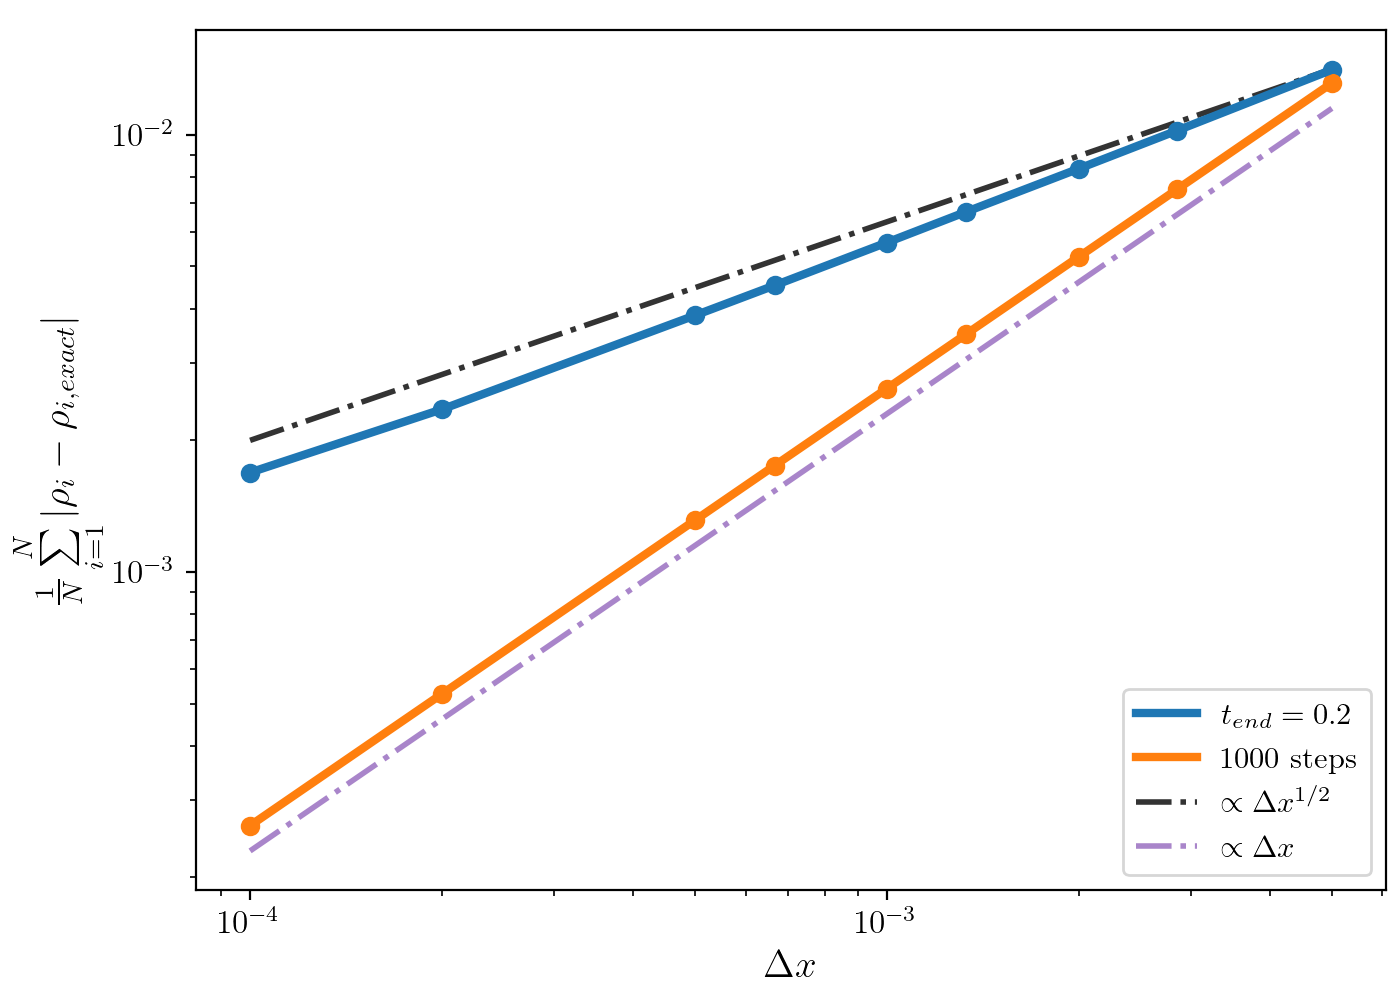
\includegraphics[width=.5\textwidth]{
    ./figures/FV/godunov_euler/accuracy_dx.png}%
    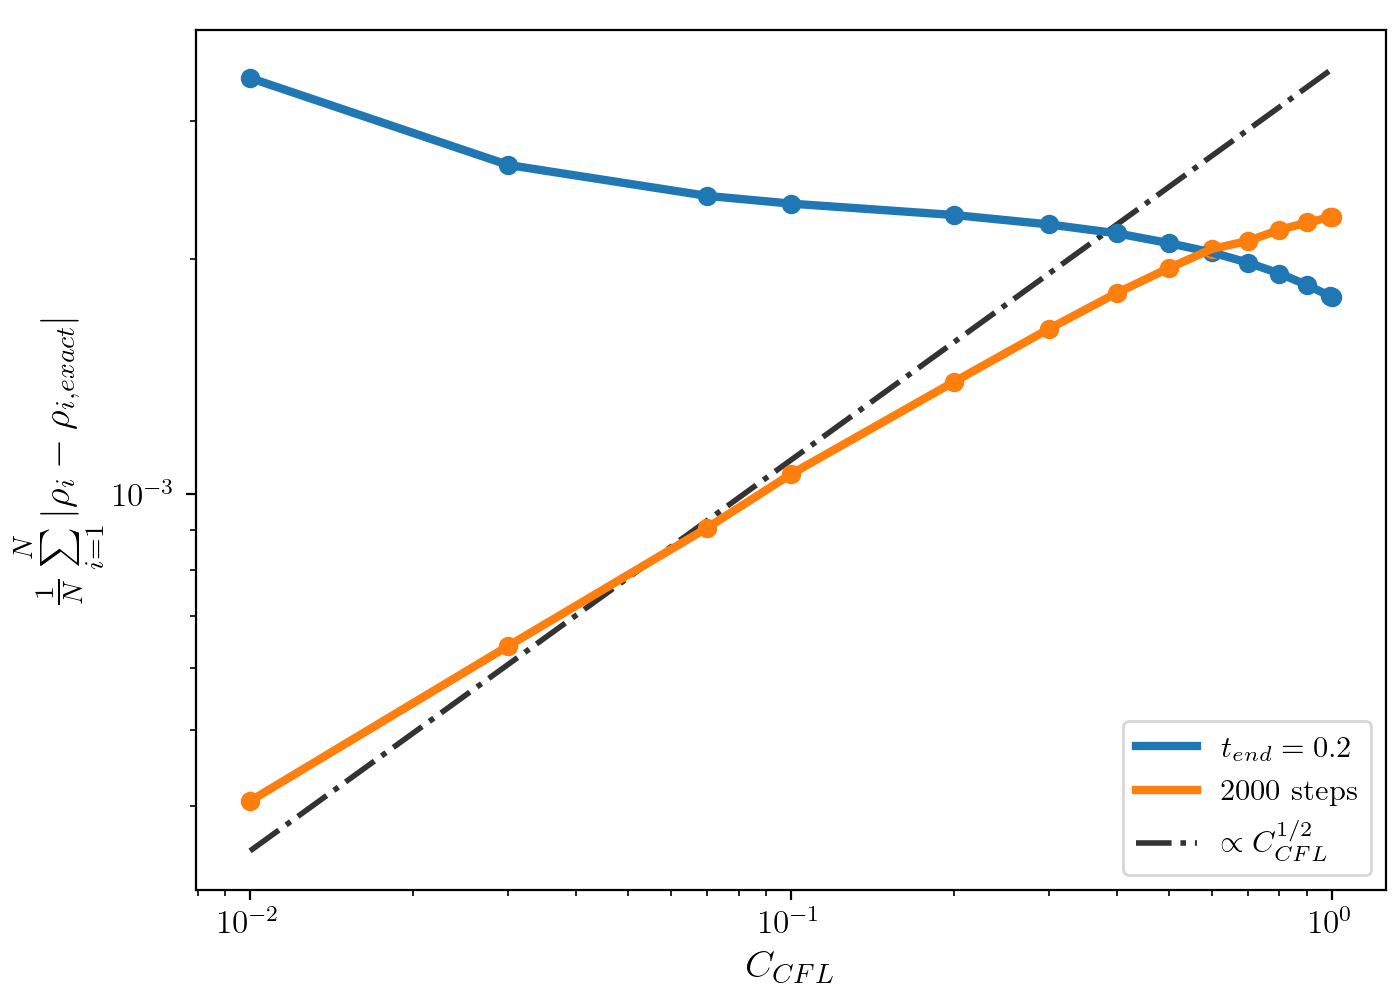
\includegraphics[width=.5\textwidth]{
    ./figures/FV/godunov_euler/accuracy_CFL.png}%
    \caption[Order of accuracy w.r.t $\Delta x$ and $C_{CFL}$ for Euler equations using Godunov's
method.]{
The order of accuracy w.r.t. $\Delta x$ (left) and the Courant number $C_{CFL}$ (right) of
the Euler equations using Godunov's method for the Sod test (eq.~\ref{eq:sod-test-ICs}). For
comparison, lines with slopes $1/2$, and $1$ are over-plotted. The experiments are run for both a
fixed end time $t_{end} = 0.2$ as well as for a fixed total number of time steps individually. The
fixed total number of steps was chosen such that all three waves remain within the boundary for all
choices of $\Delta x$ and $C_{CFL}$.
    }%
    \label{fig:godunov-accuracy}
\end{figure}















